\section{Implementation}
\newcommand{\ImplementationTitle}{Implementation}
\begin{frame}
    \frametitle{\ImplementationTitle}
    \centering
    \begin{minipage}{1\textwidth}
        \begin{itemize}%[<+->]
            \item SME introduction
            \item Processes
            \begin{itemize}
                \item State machines
            \end{itemize}
            \item Buffers
            \begin{itemize}
                \item Memory segments
                \item Dictionary
            \end{itemize}
            \item Interface signal control
            \begin{itemize}
                \item Buffer-Producer
                \item Compute-Producer
            \end{itemize}
        \end{itemize}
    \end{minipage}
\end{frame}

\begin{frame}
    \begin{textblock*}{\displayThumbnail}(\paperwidth-\displayThumbnail-0.2cm,0cm) % {block width} (coords)
        \colorbox{white}{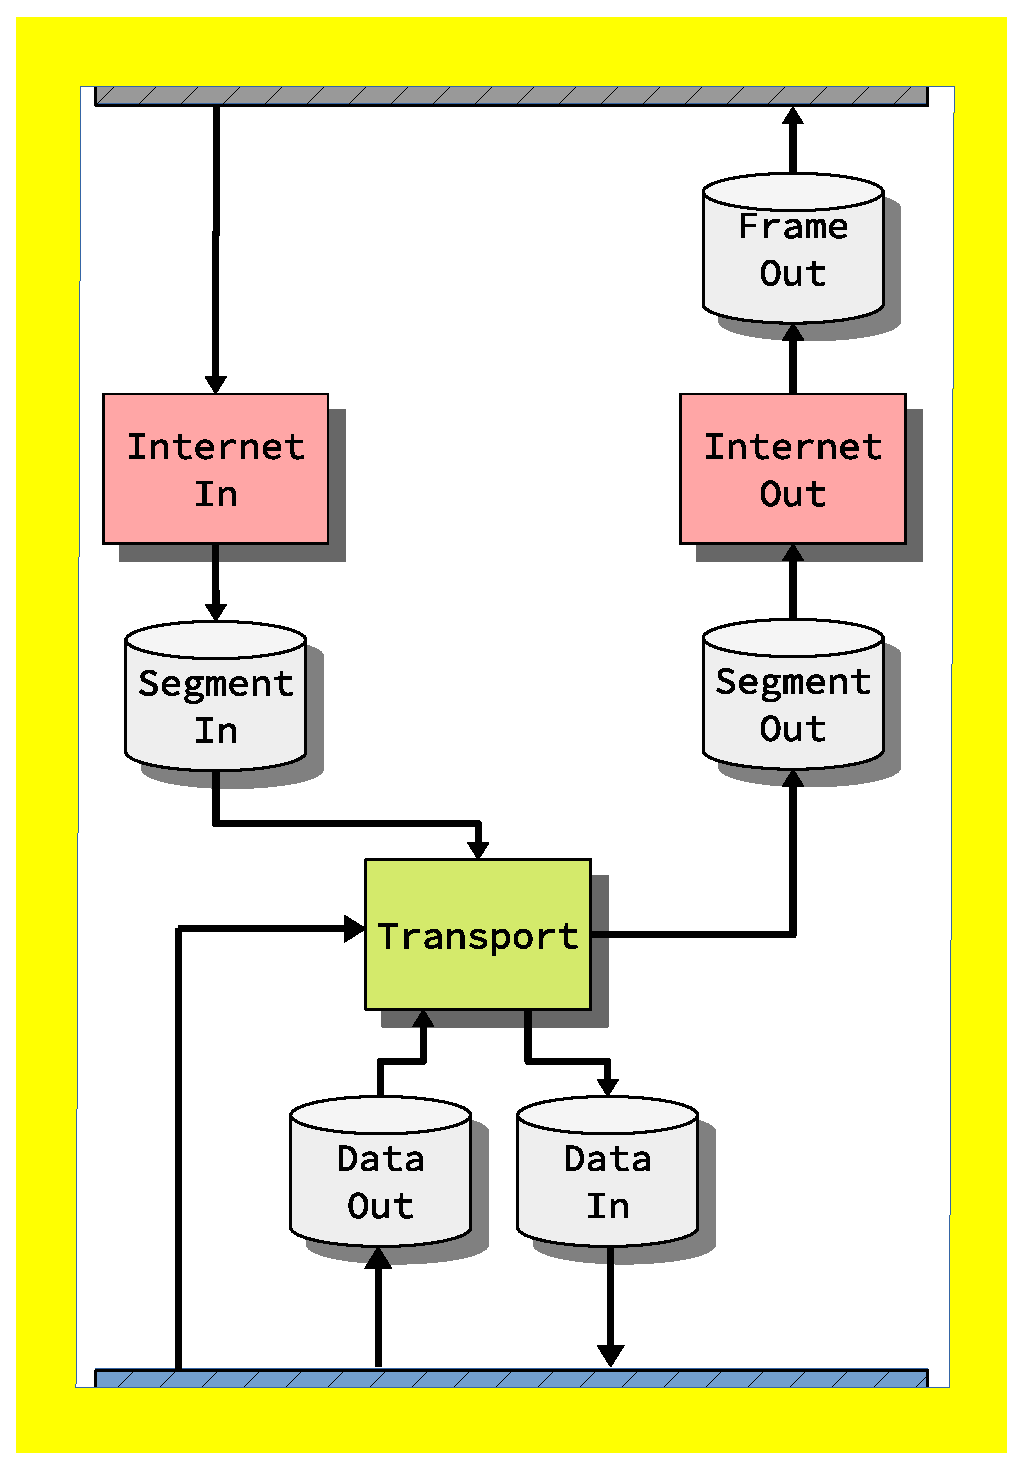
\includegraphics[width=\textwidth]{implementation/design_2_sme.eps}}
    \end{textblock*}
    \frametitle{\ImplementationTitle}
    \framesubtitle{SME introduction}
    SME(Synchronous Message Exchange) introduction
    \begin{itemize}
        \item Processes and Busses
        \item Higher abstraction
        \item Handling of clocks
        \item Easy testing
        \item Not fully feature complete with C\#(No threads, no allocation)
    \end{itemize}
\end{frame}
\note{
    \begin{itemize}
        \item What is a bus and a process
        \item No VHDL code
        \item Clocks abstracted away behind the management of processes and busses
        \item Testing straight in the simulator, but also in afterwards in the GHDL
              compiler, via an clock lookup table
    \end{itemize}
}
\begin{frame}[fragile]
    \begin{textblock*}{\displayThumbnail}(\paperwidth-\displayThumbnail-0.2cm,0cm) % {block width} (coords)
        \colorbox{white}{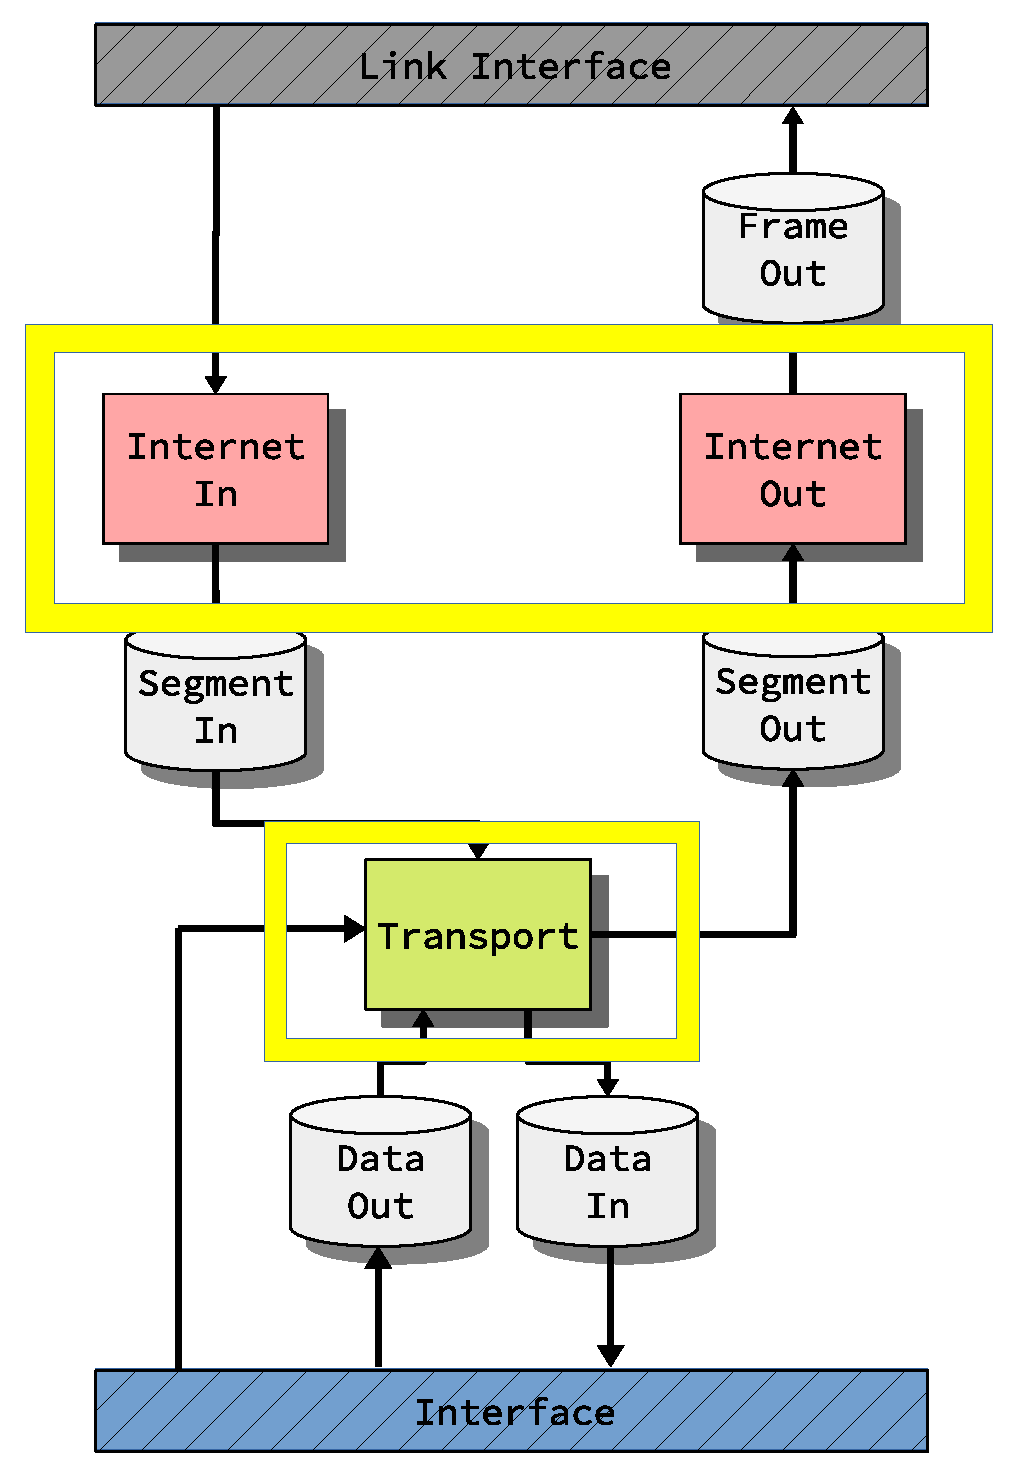
\includegraphics[width=\textwidth]{implementation/design_2_state.eps}}
    \end{textblock*}
    \frametitle{\ImplementationTitle}
    \framesubtitle{Processes}
    State machines\\\\
    %\begin{onlyenv}<2>
    \begin{minipage}[t]{0.3\textwidth}
        \begin{mintedcsharp}
            public class SomeProcess : StateProcess
            {
              private override async Task OnTickAsync()
              {
                a();
                await ClockAsync();
                b();
                await ClockAsync();
                c();
                await ClockAsync();
              }
            }
        \end{mintedcsharp}
    \end{minipage}%
    %\end{onlyenv}%
    \hfill%
    \begin{minipage}[t]{0.3\textwidth}
        \begin{mintedcsharp}
            public class SomeProcess : SimpleProcess
            {
            // Initial state
            state = A;

            protected override void OnTick()
            {
              switch(state) {
                case A:
                  a();
                  state = B;
                case B:
                  b();
                  state = C;
                case C:
                  c();
                  state = A;
              }
            }
        \end{mintedcsharp}
    \end{minipage}%
    \hfill%
    \begin{minipage}[t]{0.3\textwidth}
        \begin{figure}
                \centering
                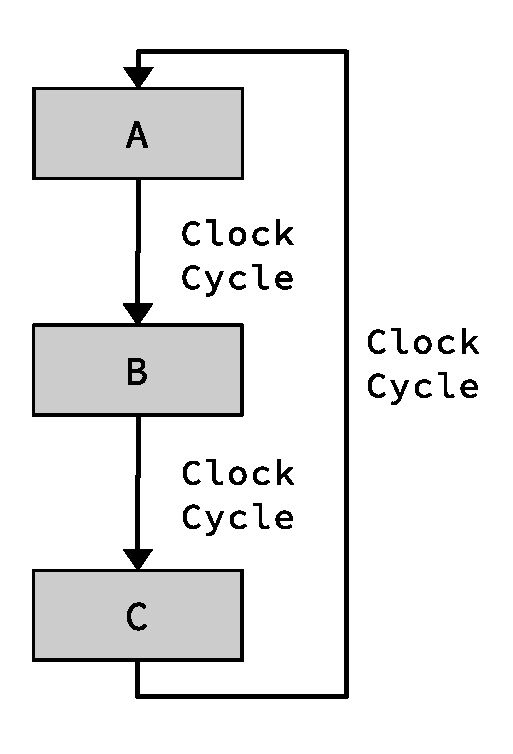
\includegraphics[scale=0.45]{implementation/empty_process_fsm.eps}
        \end{figure}
    \end{minipage}
    %\Put(-50,0){\colorbox{white}{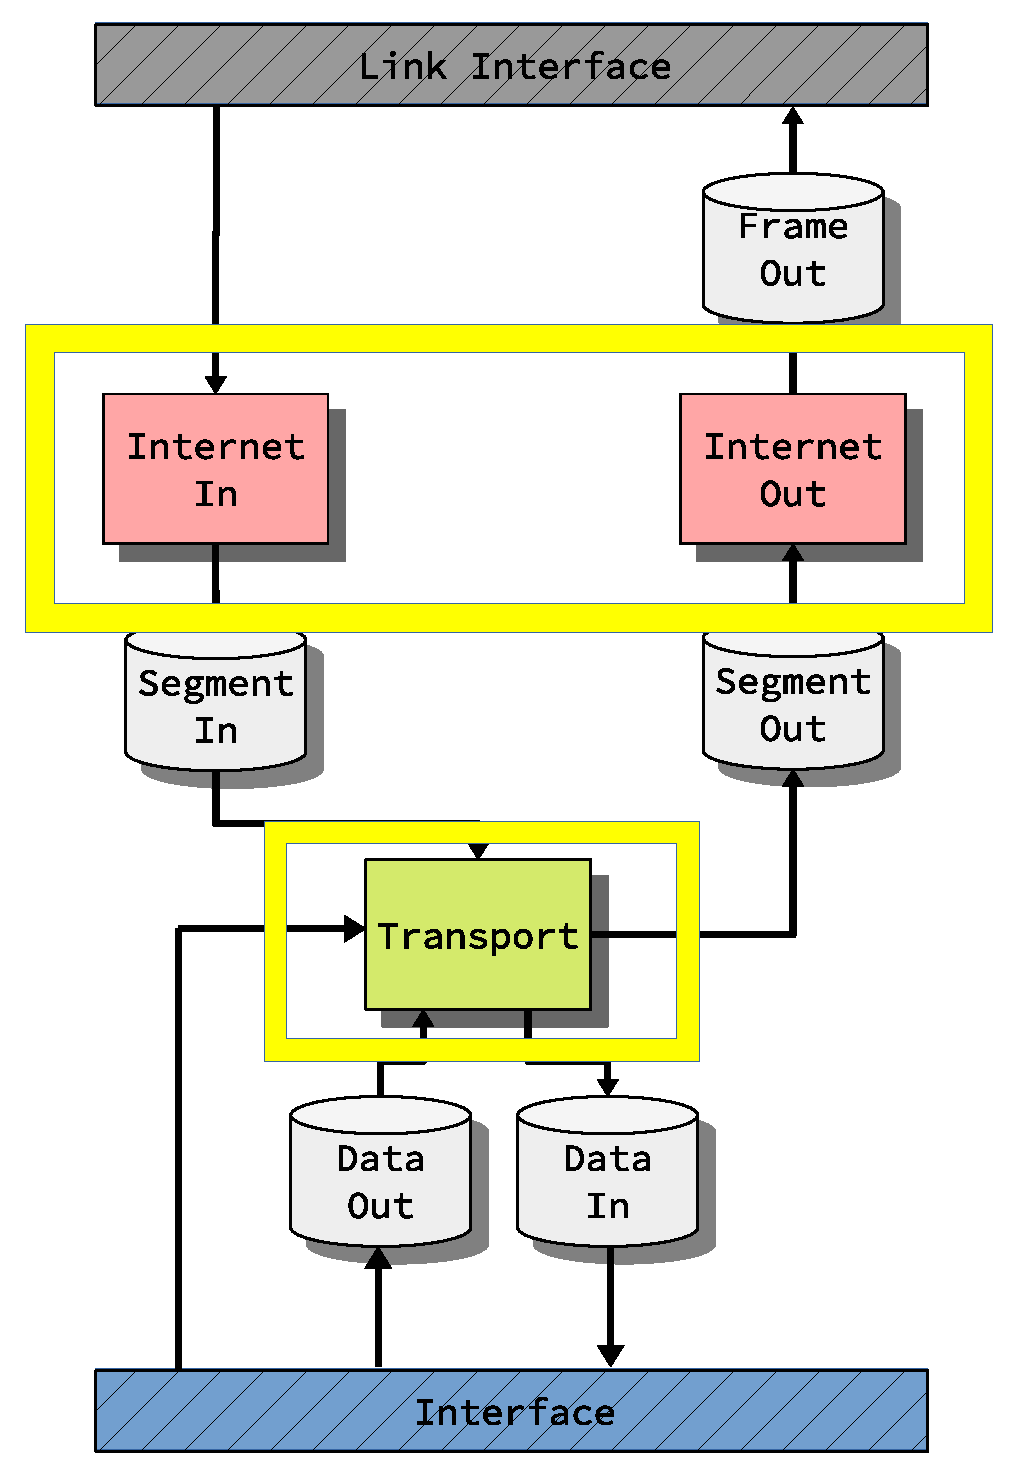
\includegraphics[width=0.2\textwidth]{implementation/design_2_state.eps}}}

\end{frame}

\note{
State machines\\
\begin{itemize}
    \item \texttt{StateProcess}\\
          Eksekvering kan stoppes når som helst(i bidder)
    \item \texttt{SimpleProcess}\\
          Run er en clock altid, state machine håndteres
          med en switchcase. Algoritme kan splittes op i flere bidder,
          men kræver en state per bid

\end{itemize}
}

\begin{frame}[fragile]
    \begin{textblock*}{\displayThumbnail}(\paperwidth-\displayThumbnail-0.2cm,0cm) % {block width} (coords)
        \colorbox{white}{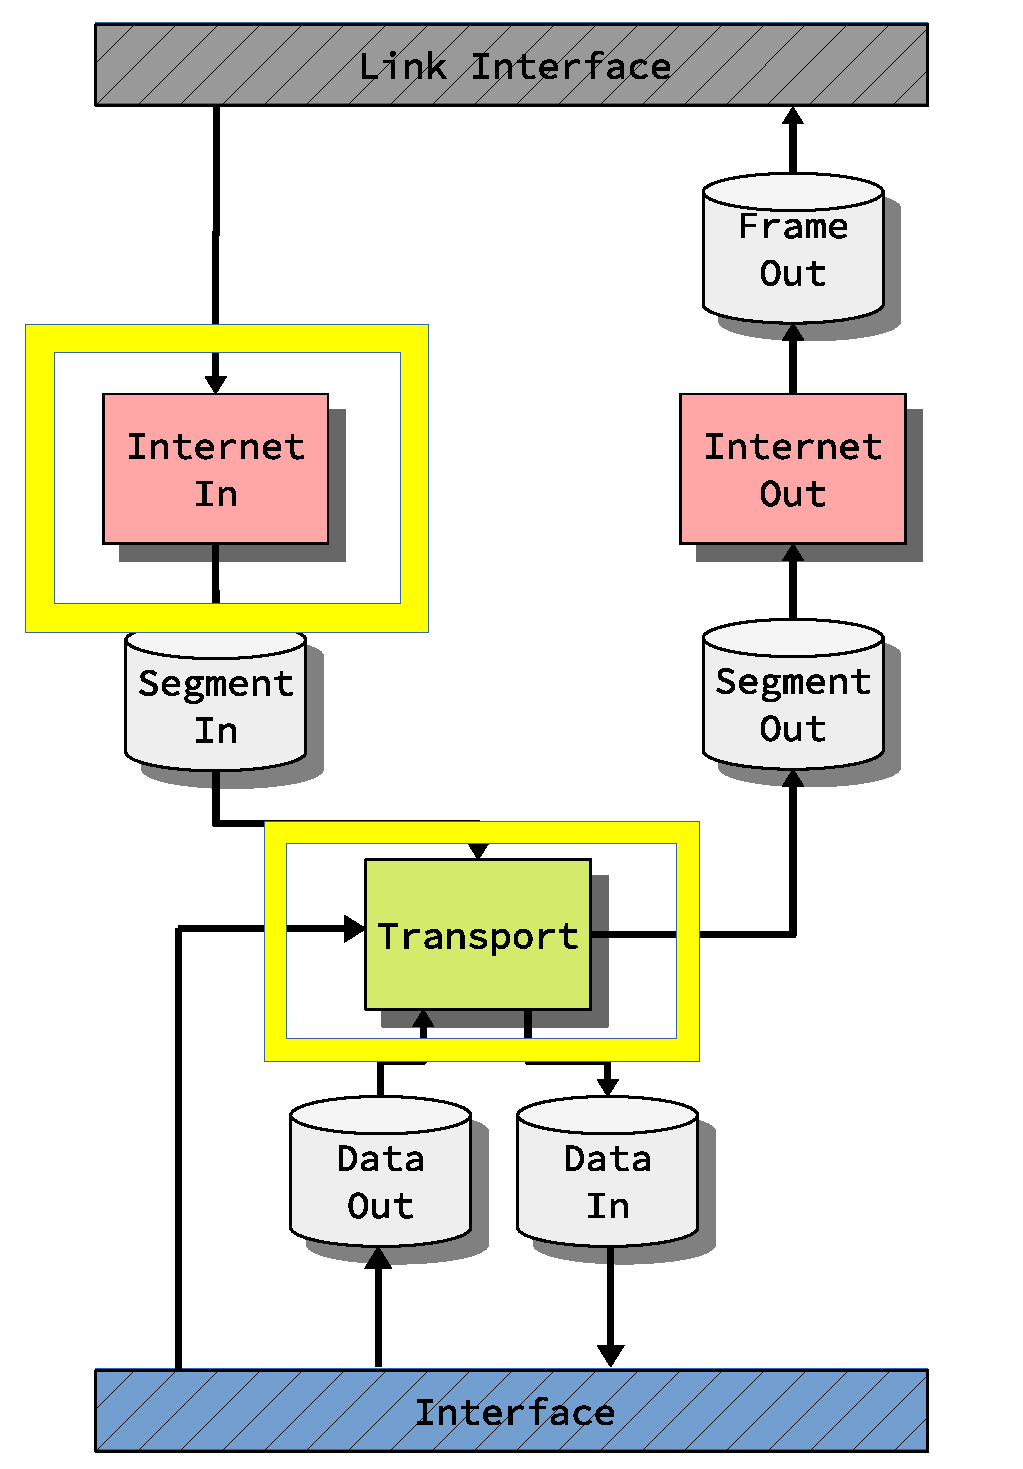
\includegraphics[width=\textwidth]{implementation/design_2_state_specific.eps}}
    \end{textblock*}
    \frametitle{\ImplementationTitle}
    \framesubtitle{Processes}
    Examples\\
    \begin{minipage}[t]{0.5\textwidth}
        \begin{figure}
            \centering
            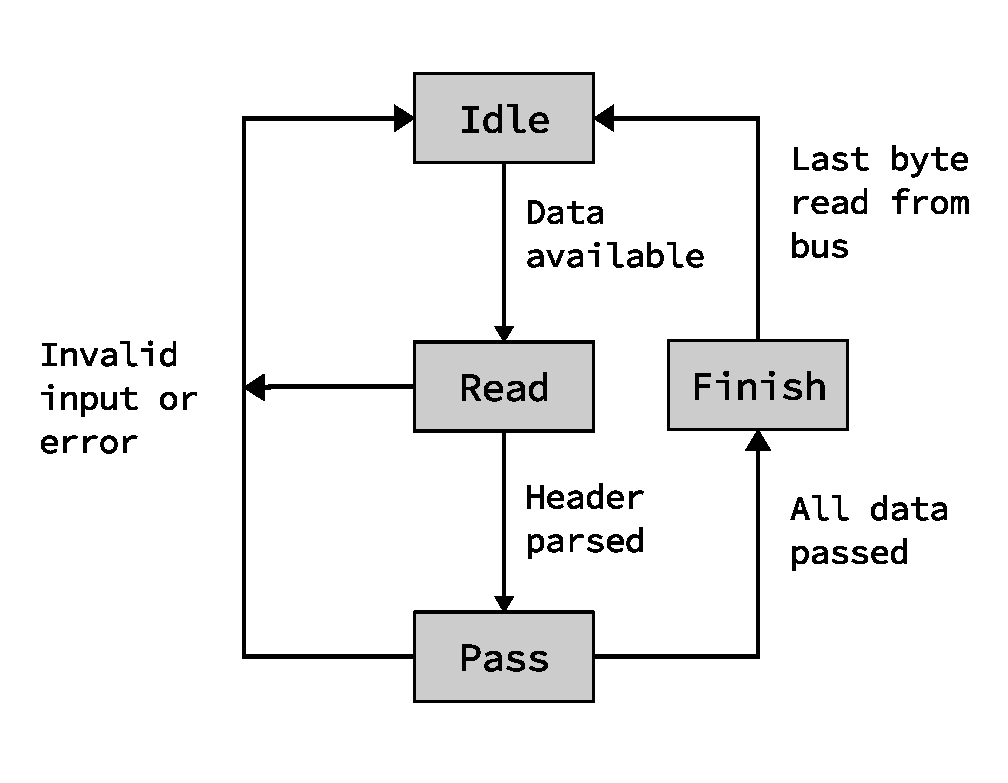
\includegraphics[scale=0.35]{implementation/internet_in_fsm.eps}
            The internet process state machine
        \end{figure}
    \end{minipage}%
    \hfill%
    \begin{minipage}[t]{0.5\textwidth}
        \begin{figure}
            \centering
            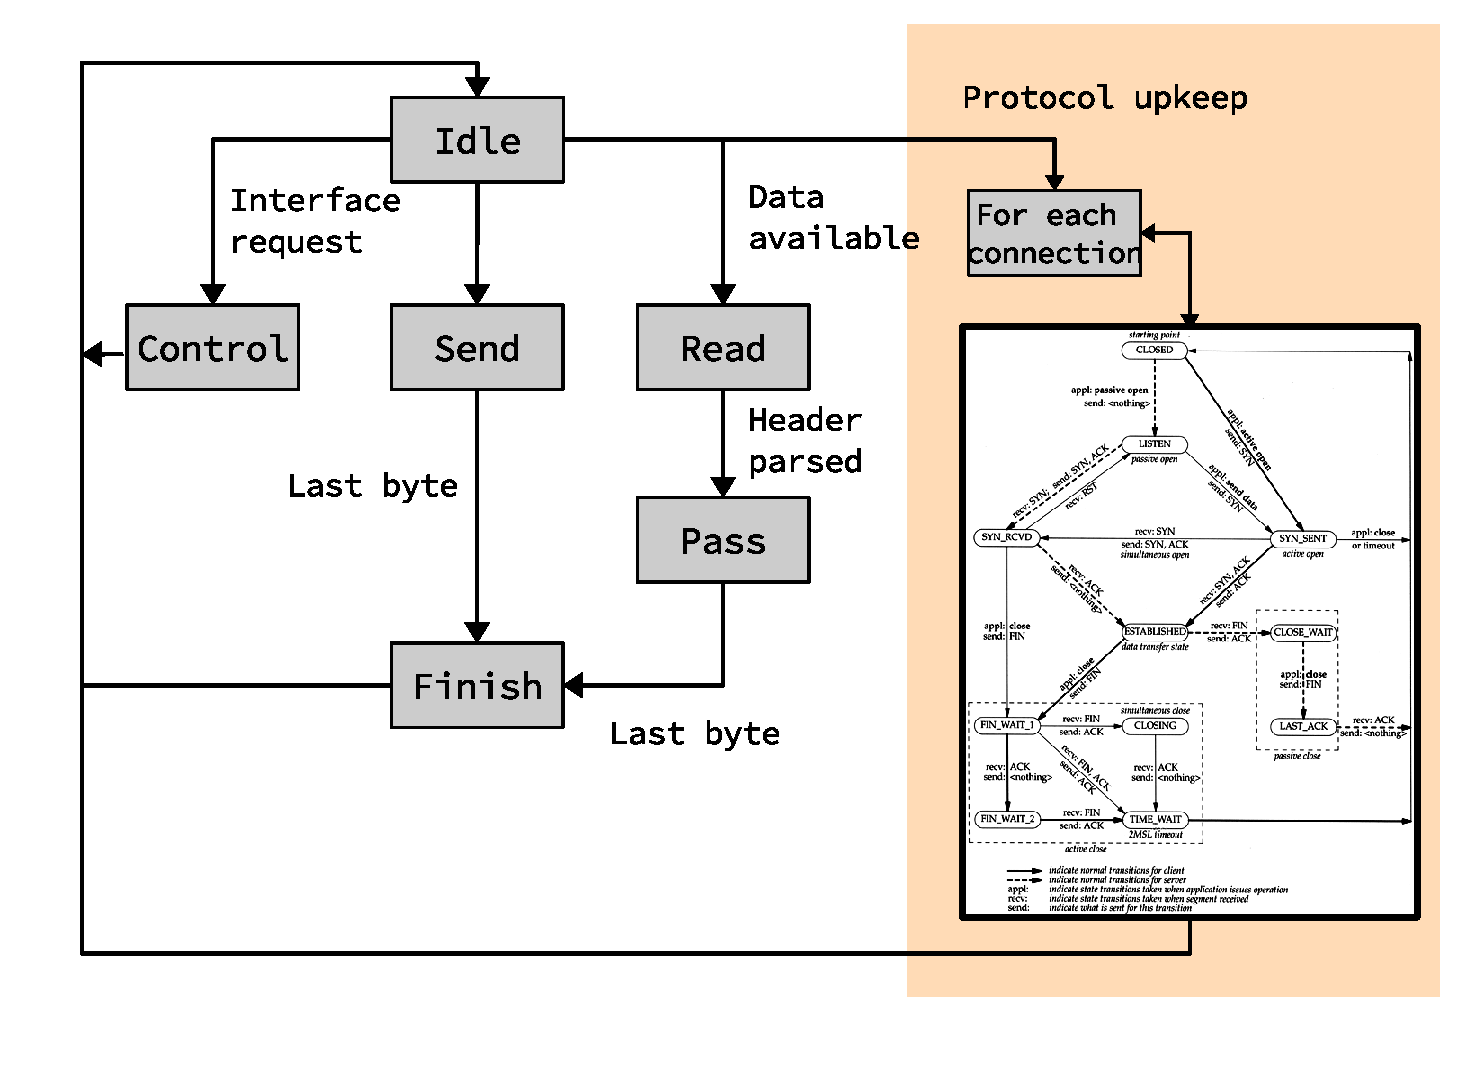
\includegraphics[scale=0.35]{implementation/transport_fsm.eps}
            The transport process state machine
        \end{figure}
    \end{minipage}
\end{frame}
\note{Labels!}

\begin{frame}[fragile]
    \begin{textblock*}{\displayThumbnail}(\paperwidth-\displayThumbnail-0.2cm,0cm) % {block width} (coords)
        \colorbox{white}{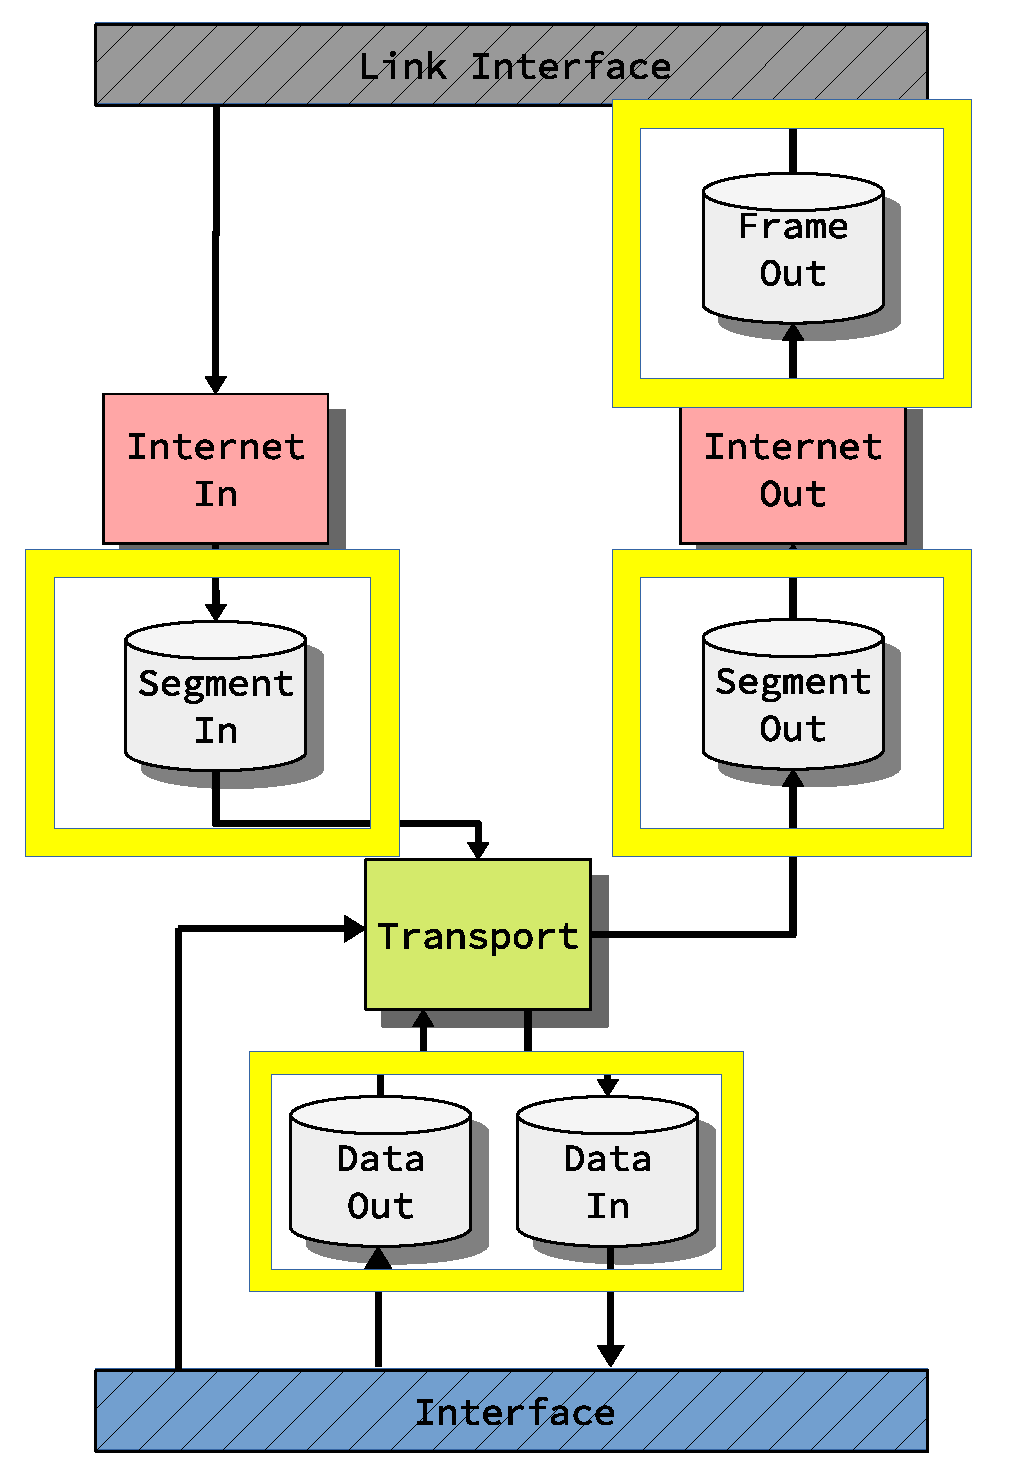
\includegraphics[width=\textwidth]{implementation/design_2_memory.eps}}
    \end{textblock*}
    \frametitle{\ImplementationTitle}
    \framesubtitle{Buffers}
    \begin{itemize}
        \item why buffes?
    \end{itemize}
\end{frame}
\note{Hvorfor bruer vi buffers?}


\begin{frame}[fragile]
    \begin{textblock*}{\displayThumbnail}(\paperwidth-\displayThumbnail-0.2cm,0cm) % {block width} (coords)
        \colorbox{white}{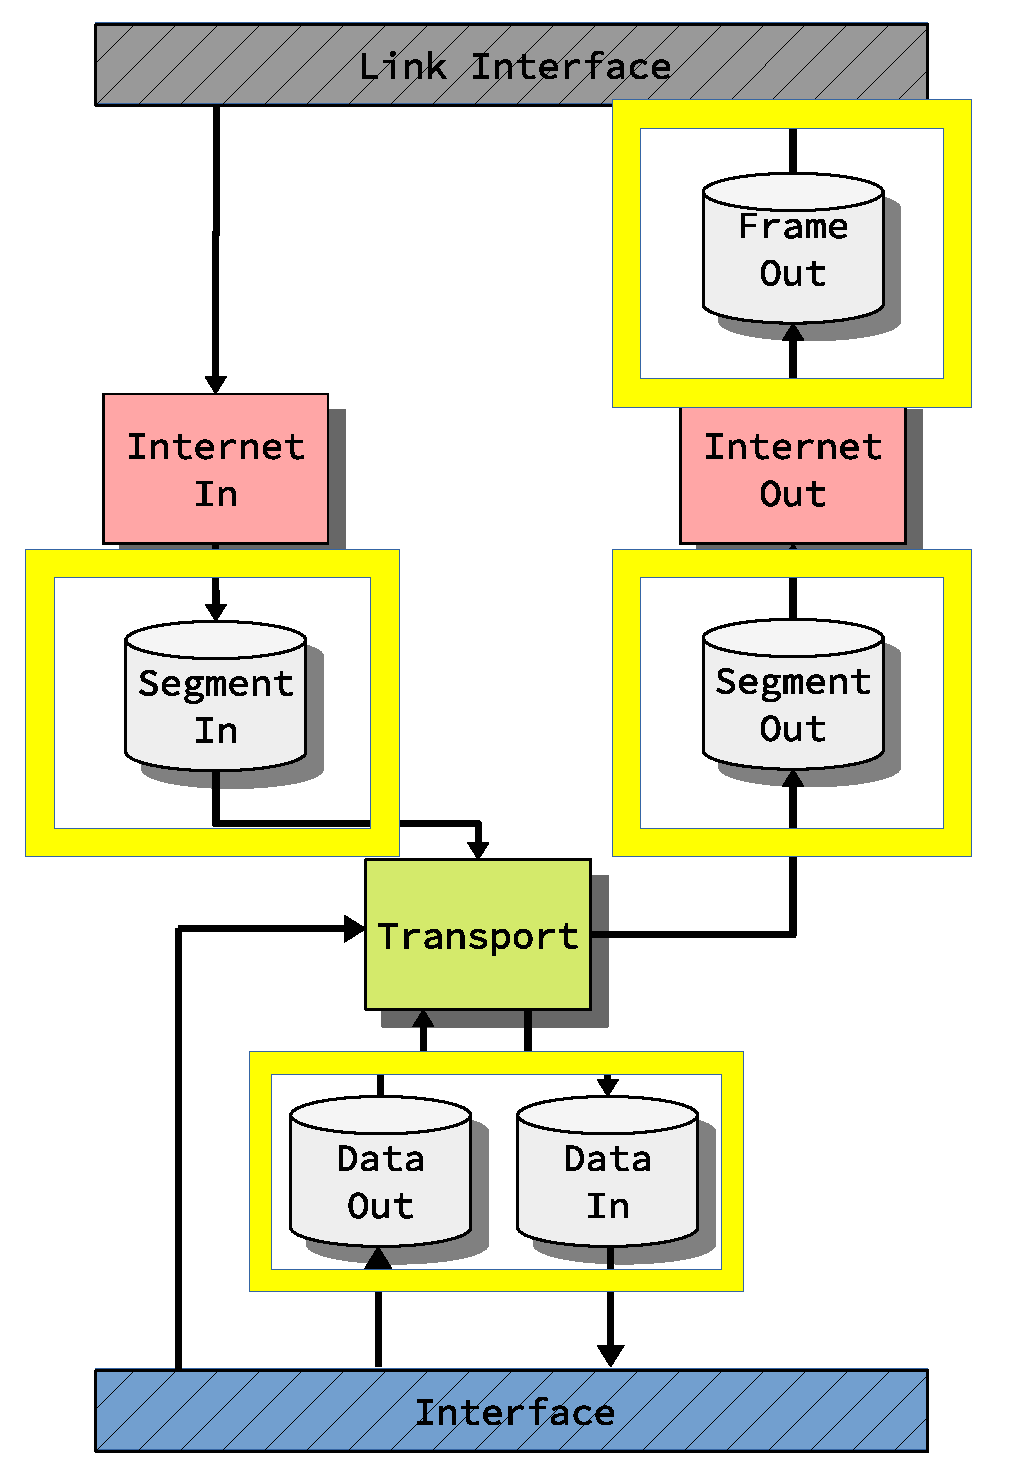
\includegraphics[width=\textwidth]{implementation/design_2_memory.eps}}
    \end{textblock*}
    \frametitle{\ImplementationTitle}
    \framesubtitle{Buffers}
    Memory segments\\
    \begin{minipage}[t]{1\textwidth}
        \begin{figure}
                \centering
                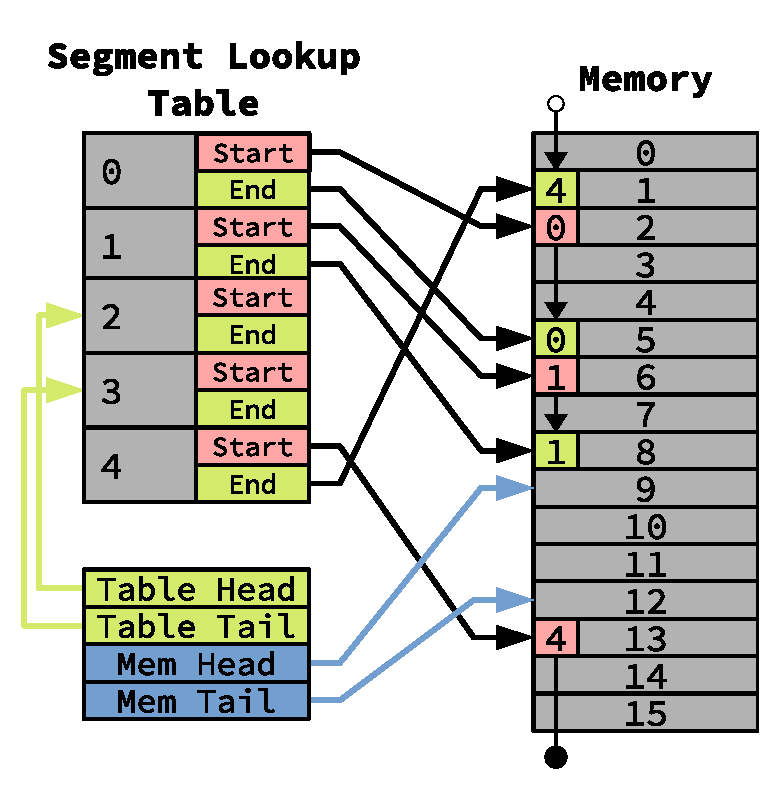
\includegraphics[scale=0.50]{implementation/memory_segments.eps}
        \end{figure}
    \end{minipage}
\end{frame}
\note{Thumbnail?}

\begin{frame}[fragile]
    \begin{textblock*}{\displayThumbnail}(\paperwidth-\displayThumbnail-0.2cm,0cm) % {block width} (coords)
        \colorbox{white}{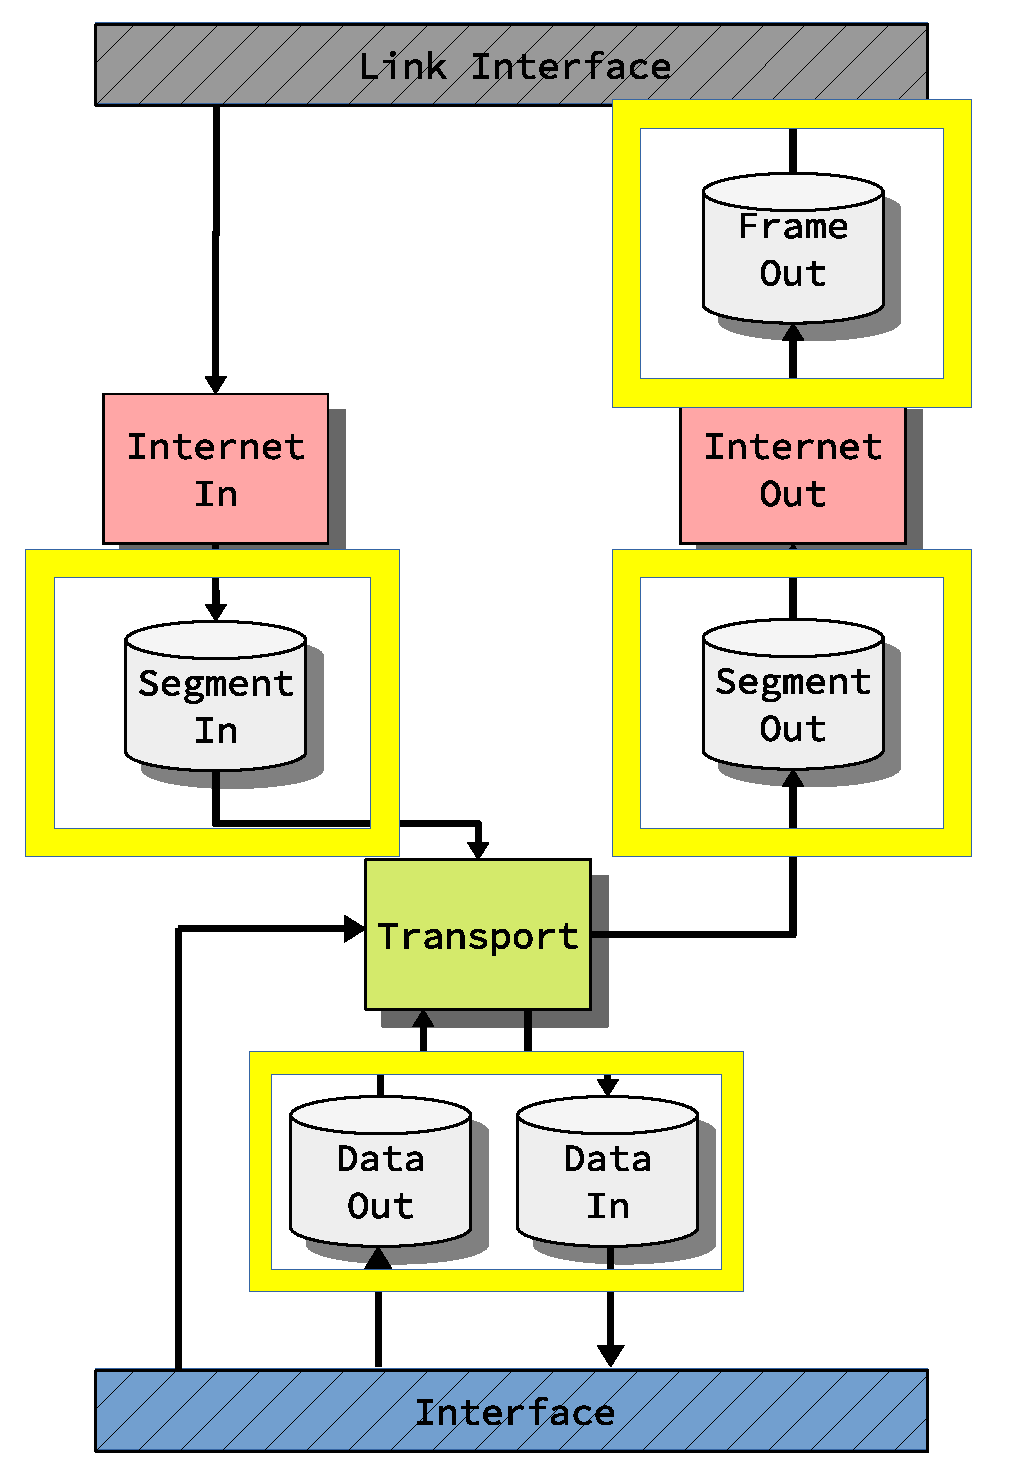
\includegraphics[width=\textwidth]{implementation/design_2_memory.eps}}
    \end{textblock*}
    \frametitle{\ImplementationTitle}
    \framesubtitle{Buffers}
    Memory dictionary\\
    \begin{minipage}[t]{1\textwidth}
        \begin{figure}
                \centering
                \includegraphics[scale=0.60]{implementation/memory_dictionary.eps}
        \end{figure}
    \end{minipage}
\end{frame}
\note{Statisk tabel?\\
Animationer?
Billede af splitup af pakker?
Hold det uden protocol specifik info.
}

\begin{frame}[fragile]
    \begin{textblock*}{\displayThumbnail}(\paperwidth-\displayThumbnail-0.2cm,0cm) % {block width} (coords)
        \colorbox{white}{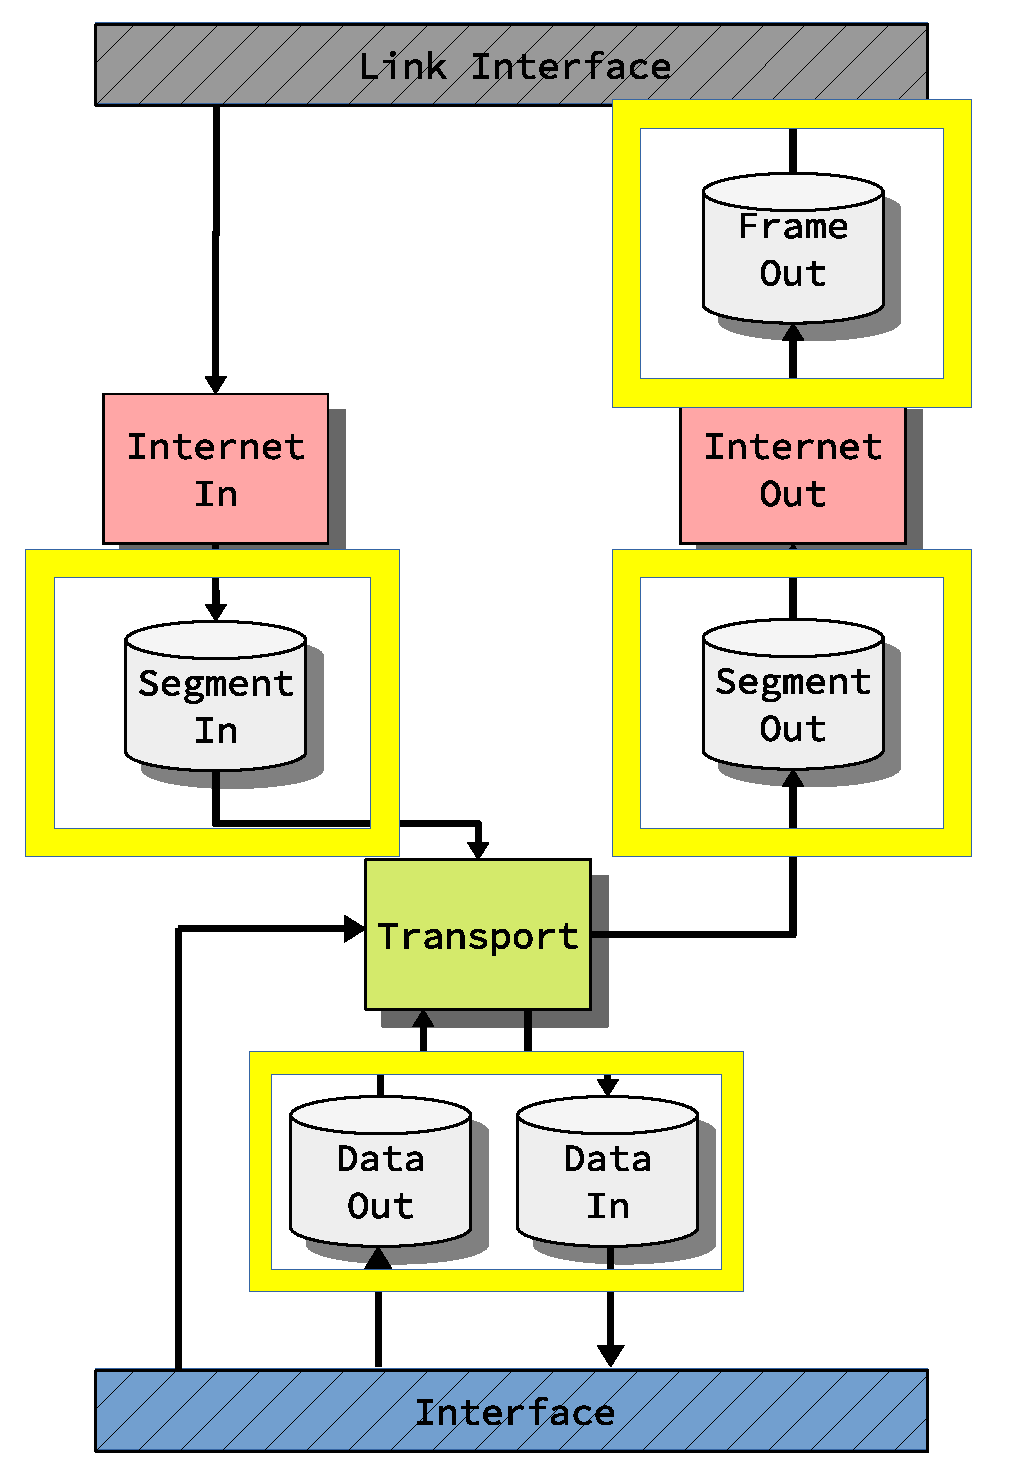
\includegraphics[width=\textwidth]{implementation/design_2_memory.eps}}
    \end{textblock*}
    \frametitle{\ImplementationTitle}
    \framesubtitle{Buffers}
    Some problems with the memory dictionaries!
    \begin{figure}[ht]
        \centering
        \begin{overlayarea}{0.76\textwidth}{\textheight}
            \only<1>{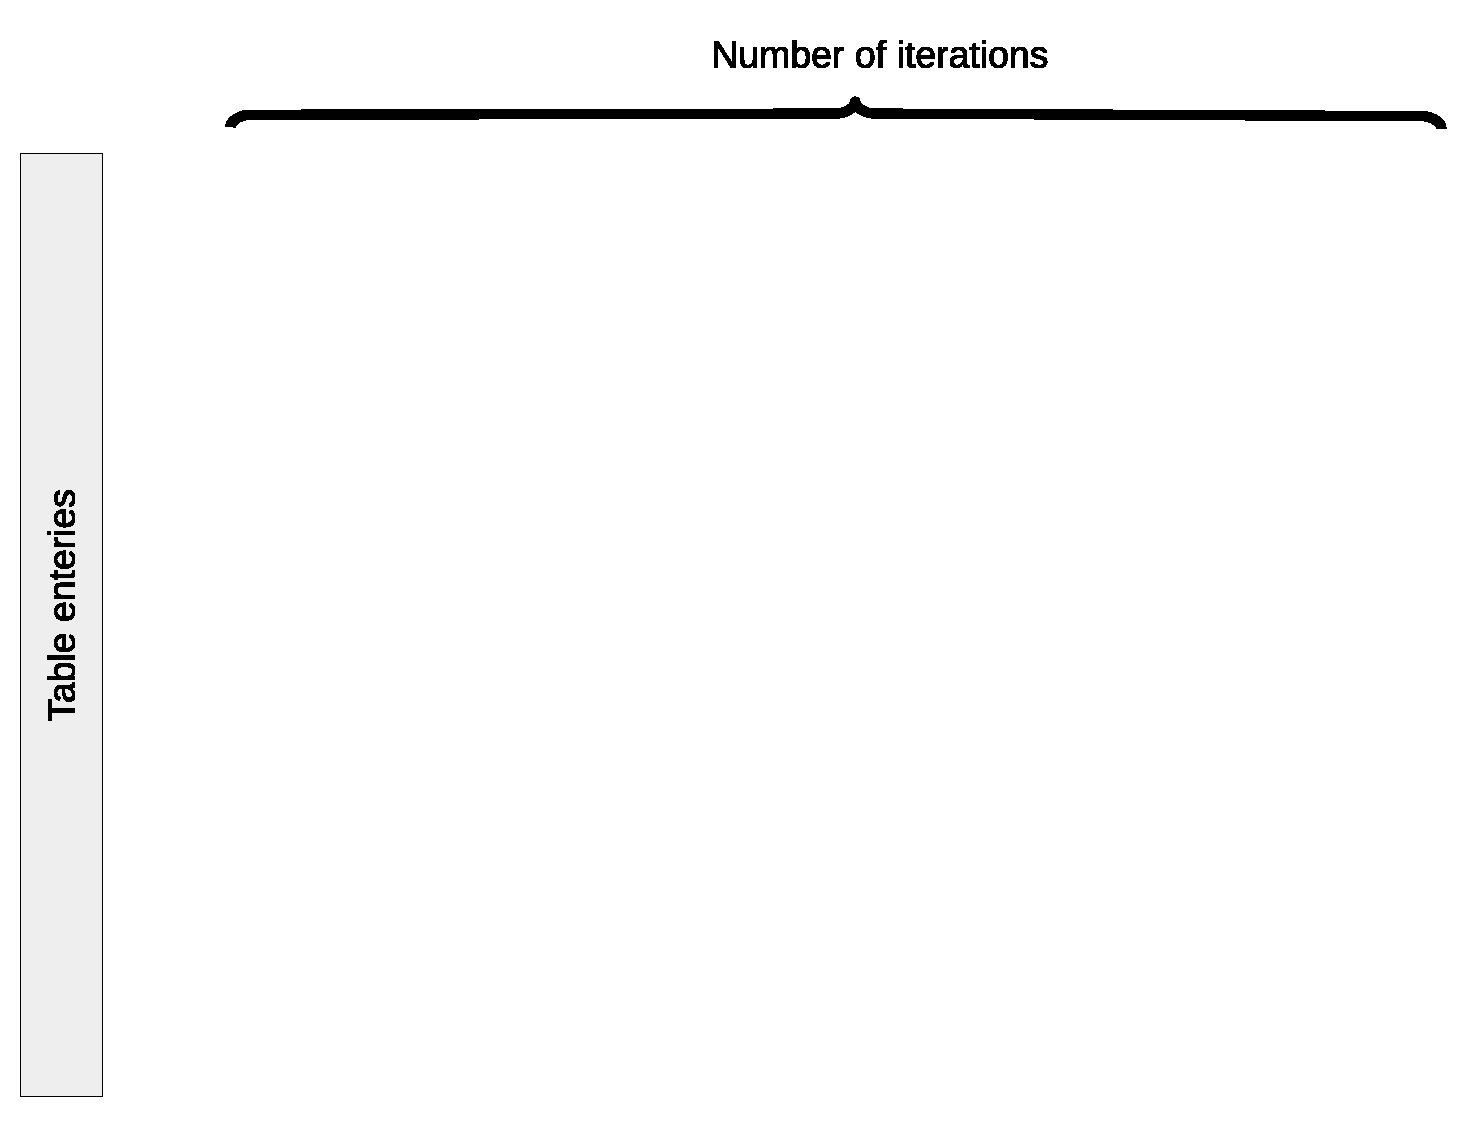
\includegraphics[width=\textwidth]{./implementation/memory_overrun/memory_overrun_0.eps}}
            \only<2>{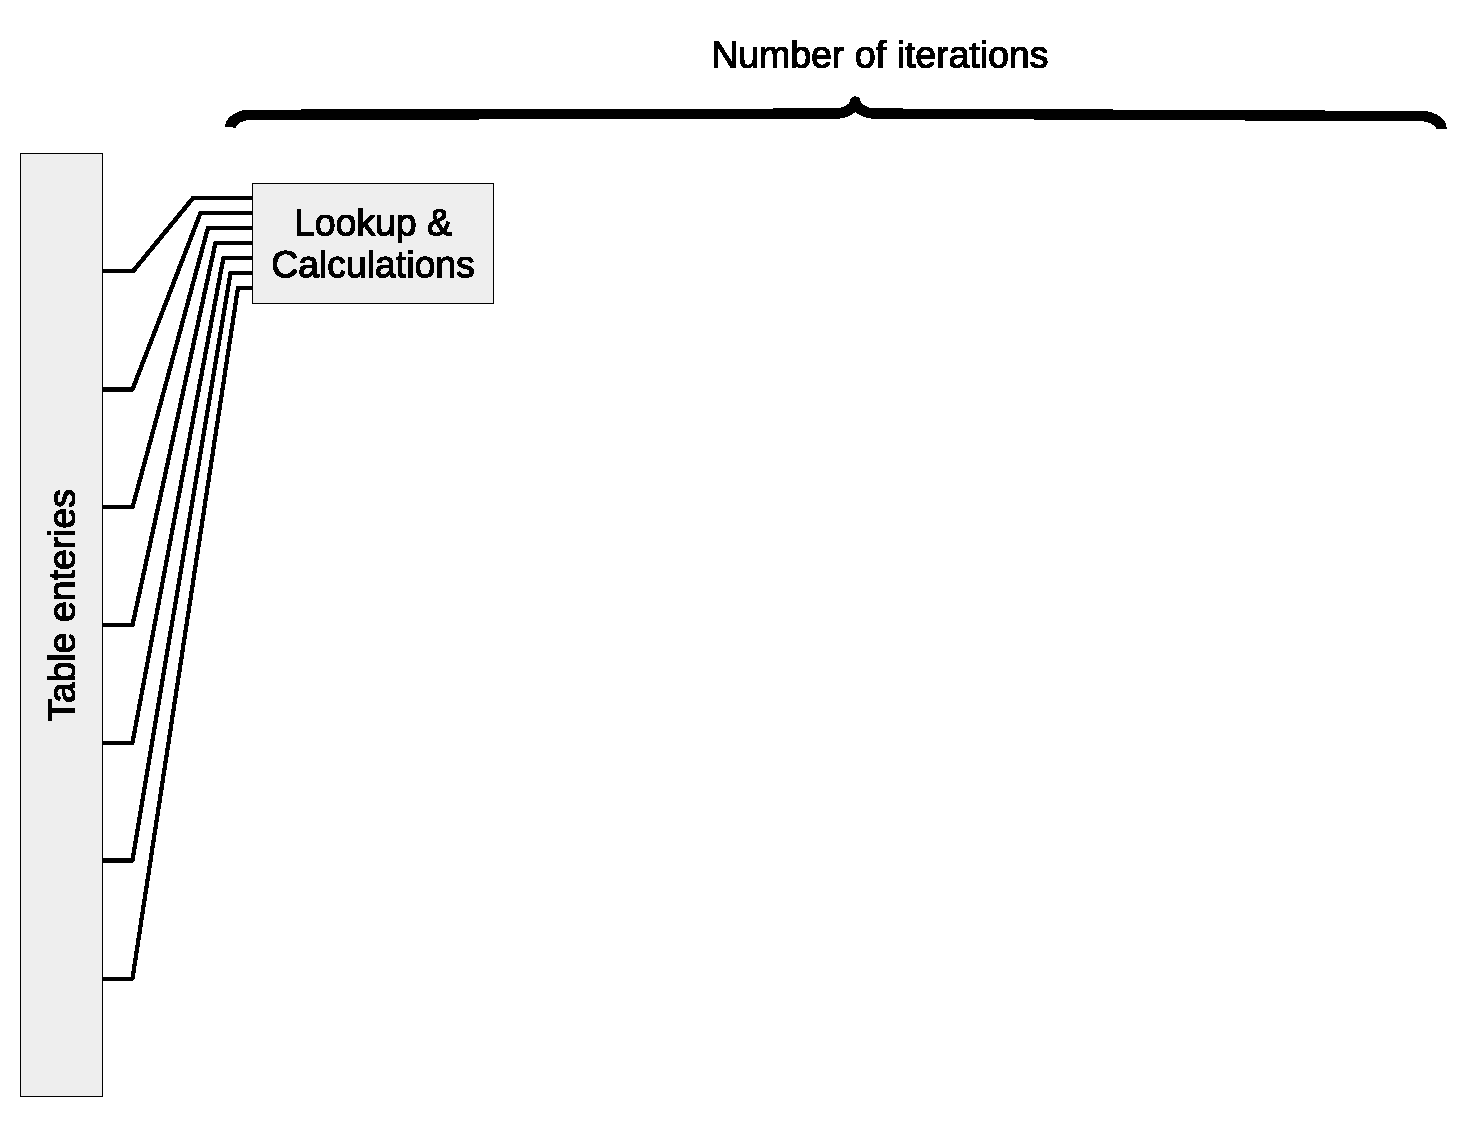
\includegraphics[width=\textwidth]{./implementation/memory_overrun/memory_overrun_1.eps}}%
            \only<3>{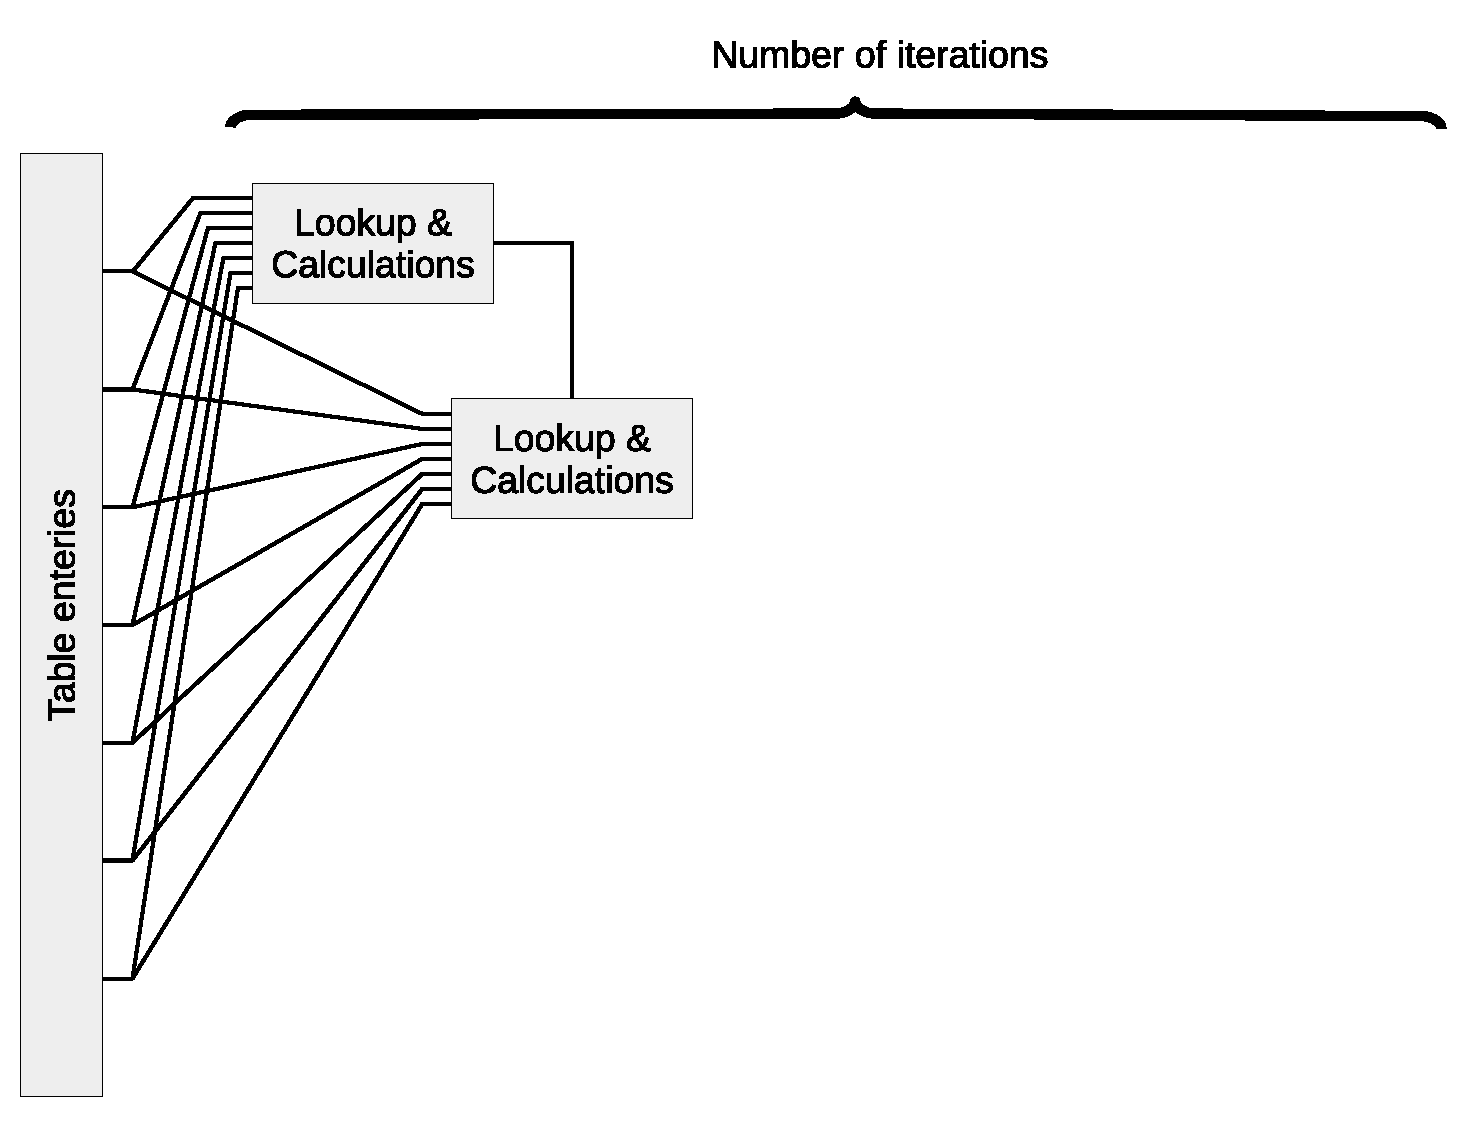
\includegraphics[width=\textwidth]{./implementation/memory_overrun/memory_overrun_2.eps}}%
            \only<4>{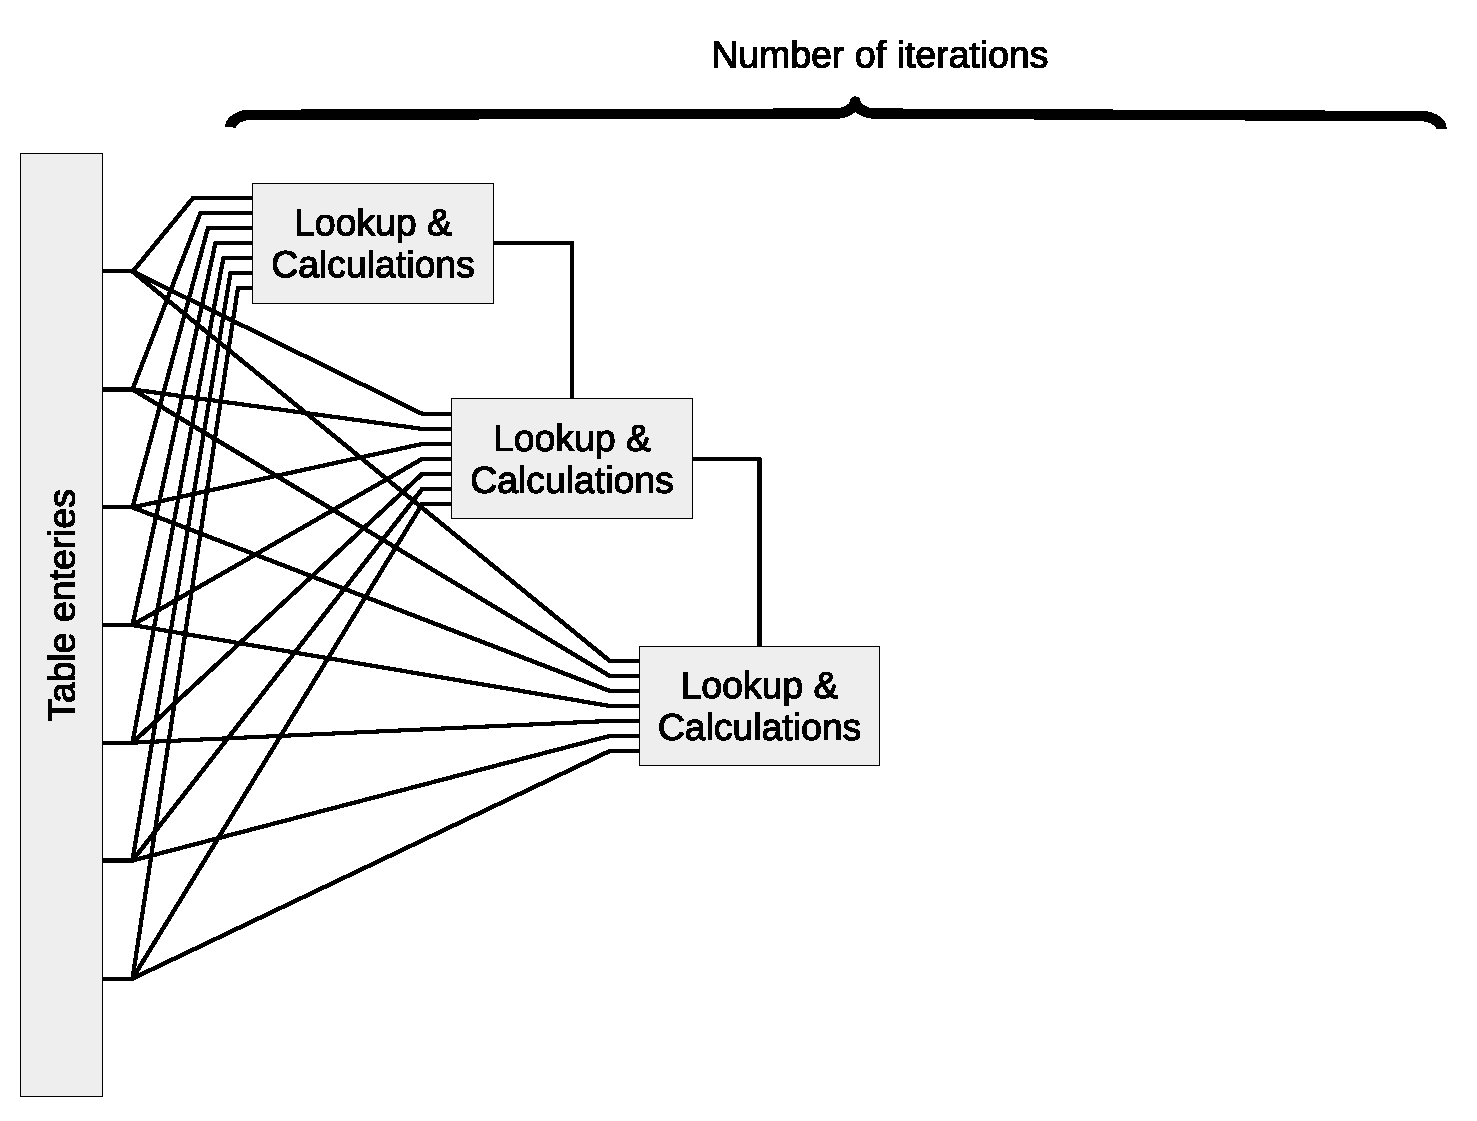
\includegraphics[width=\textwidth]{./implementation/memory_overrun/memory_overrun_3.eps}}%
            \only<5>{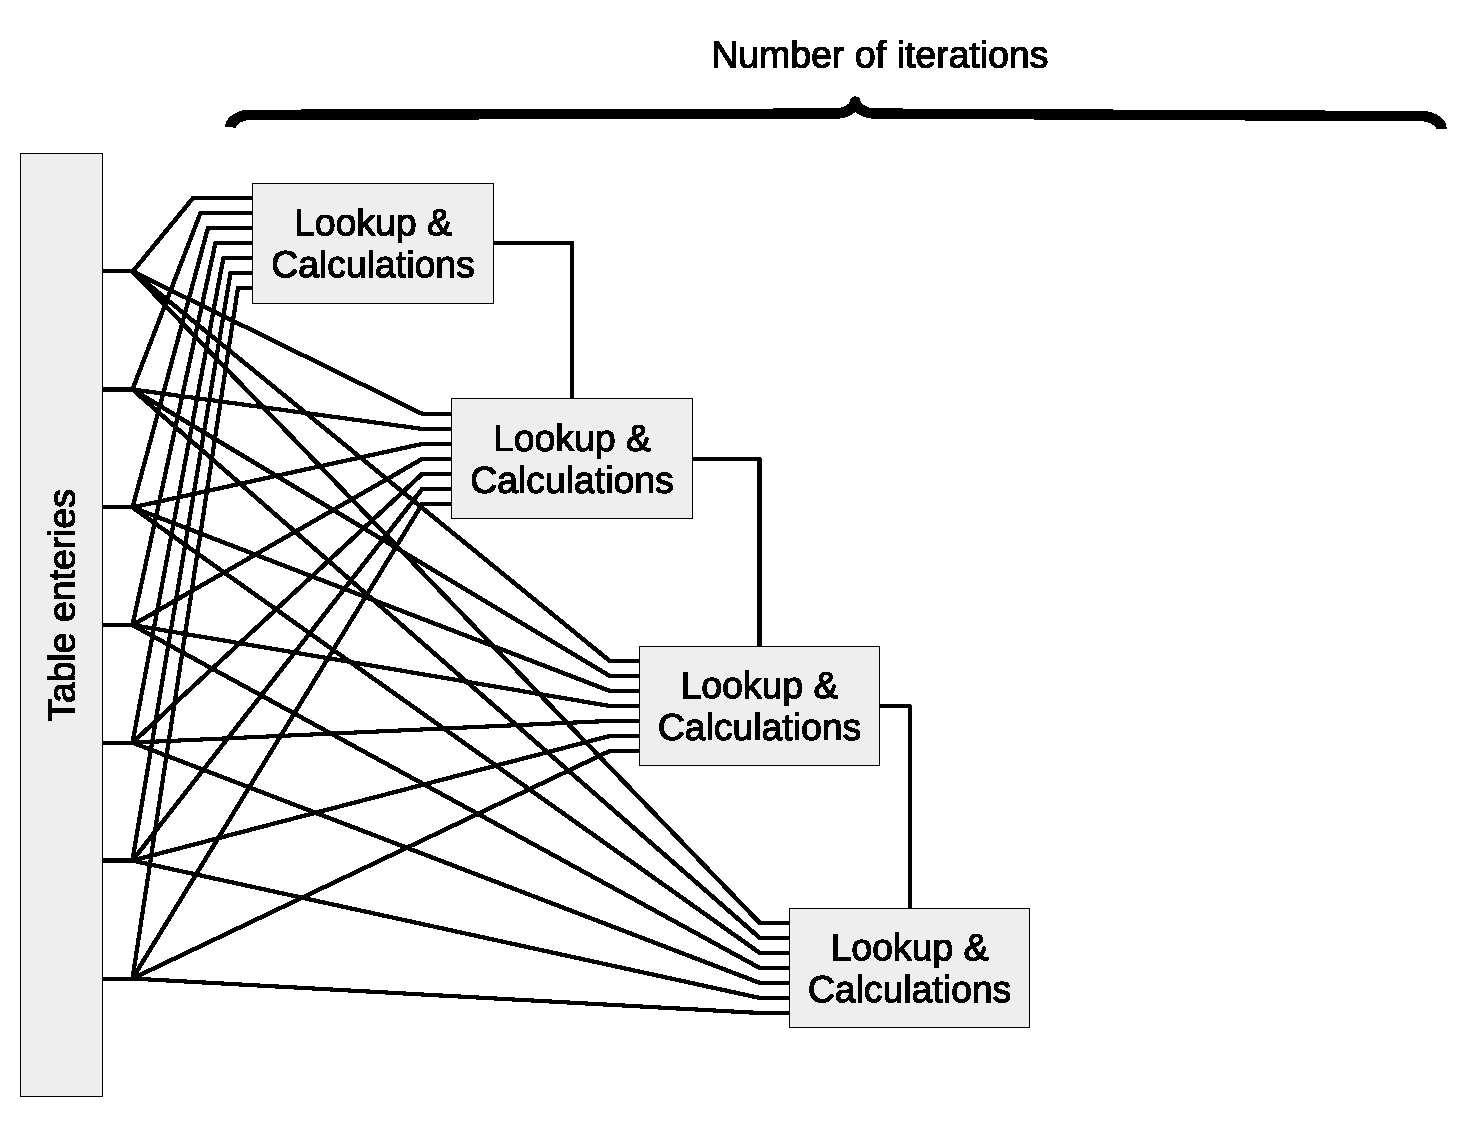
\includegraphics[width=\textwidth]{./implementation/memory_overrun/memory_overrun_4.eps}}%
            \only<6>{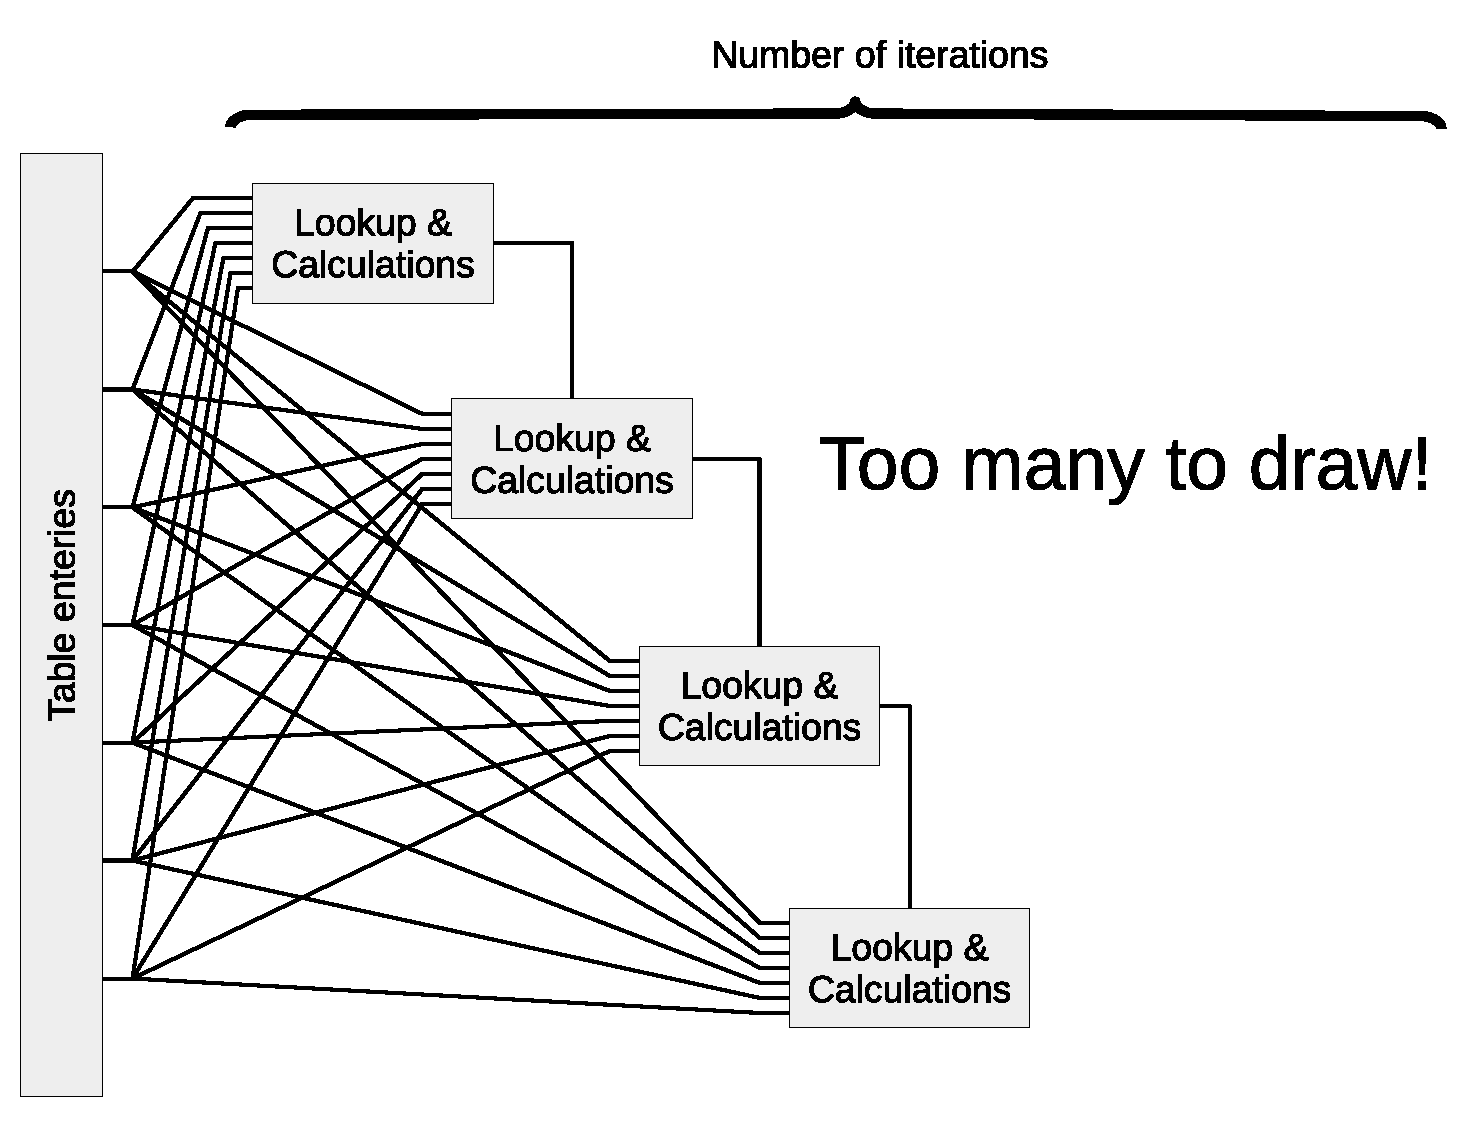
\includegraphics[width=\textwidth]{./implementation/memory_overrun/memory_overrun_5.eps}}%
        \end{overlayarea}
    \end{figure}
\end{frame}


\begin{frame}[fragile]
    \begin{textblock*}{\displayThumbnail}(\paperwidth-\displayThumbnail-0.2cm,0cm) % {block width} (coords)
        \colorbox{white}{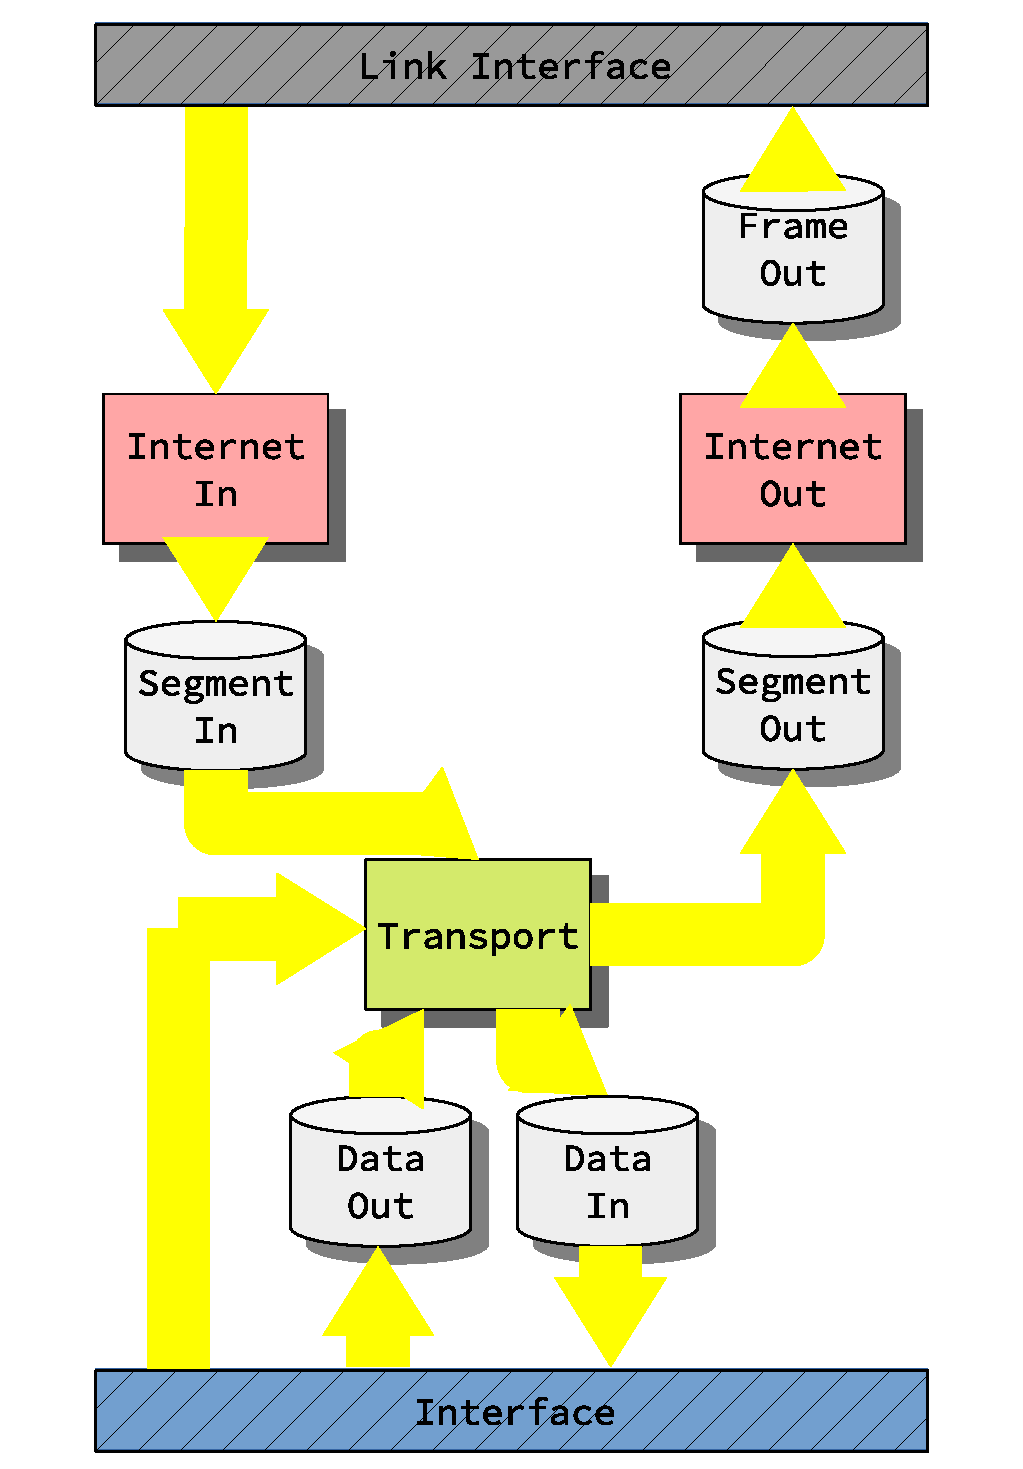
\includegraphics[width=\textwidth]{implementation/design_2_busses.eps}}
    \end{textblock*}
    \frametitle{\ImplementationTitle}
    \framesubtitle{Interface signal protocol}
Identifying the scenarios

\centering
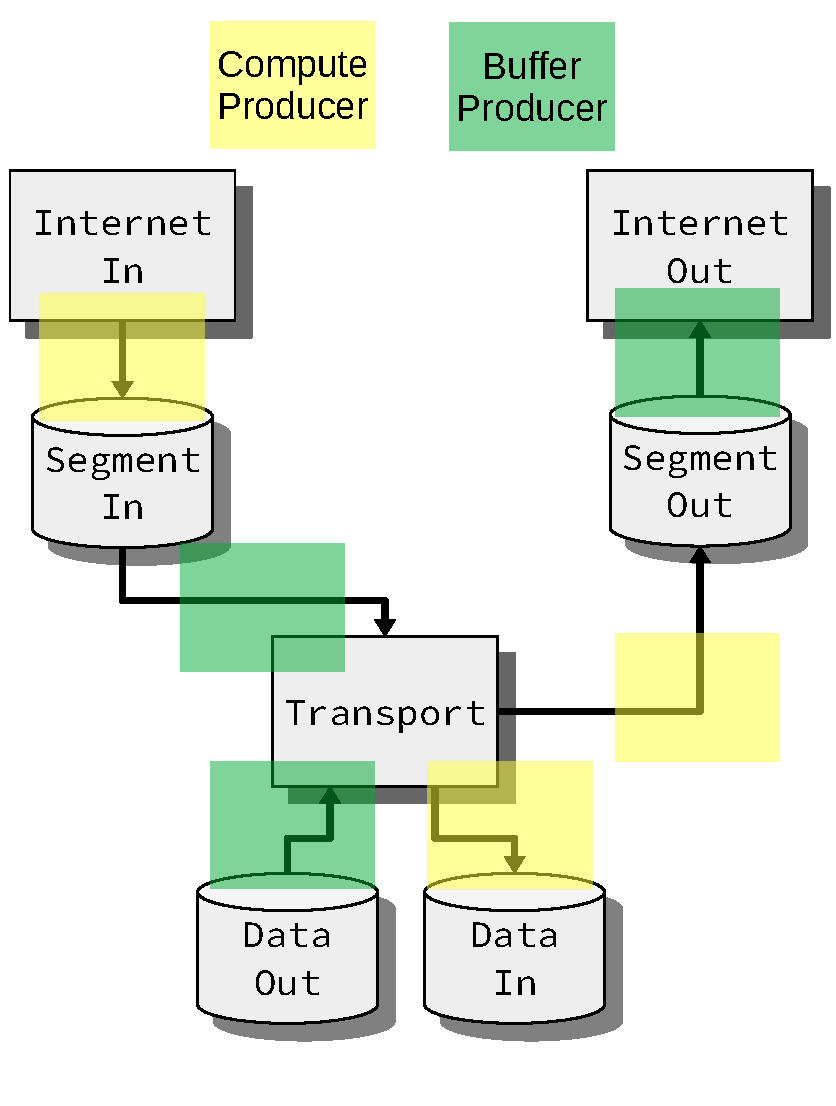
\includegraphics[scale=0.40]{implementation/signal_protocol_identification.pdf}

\end{frame}

\begin{frame}[fragile]
    \begin{textblock*}{\displayThumbnail}(\paperwidth-\displayThumbnail-0.2cm,0cm) % {block width} (coords)
        \colorbox{white}{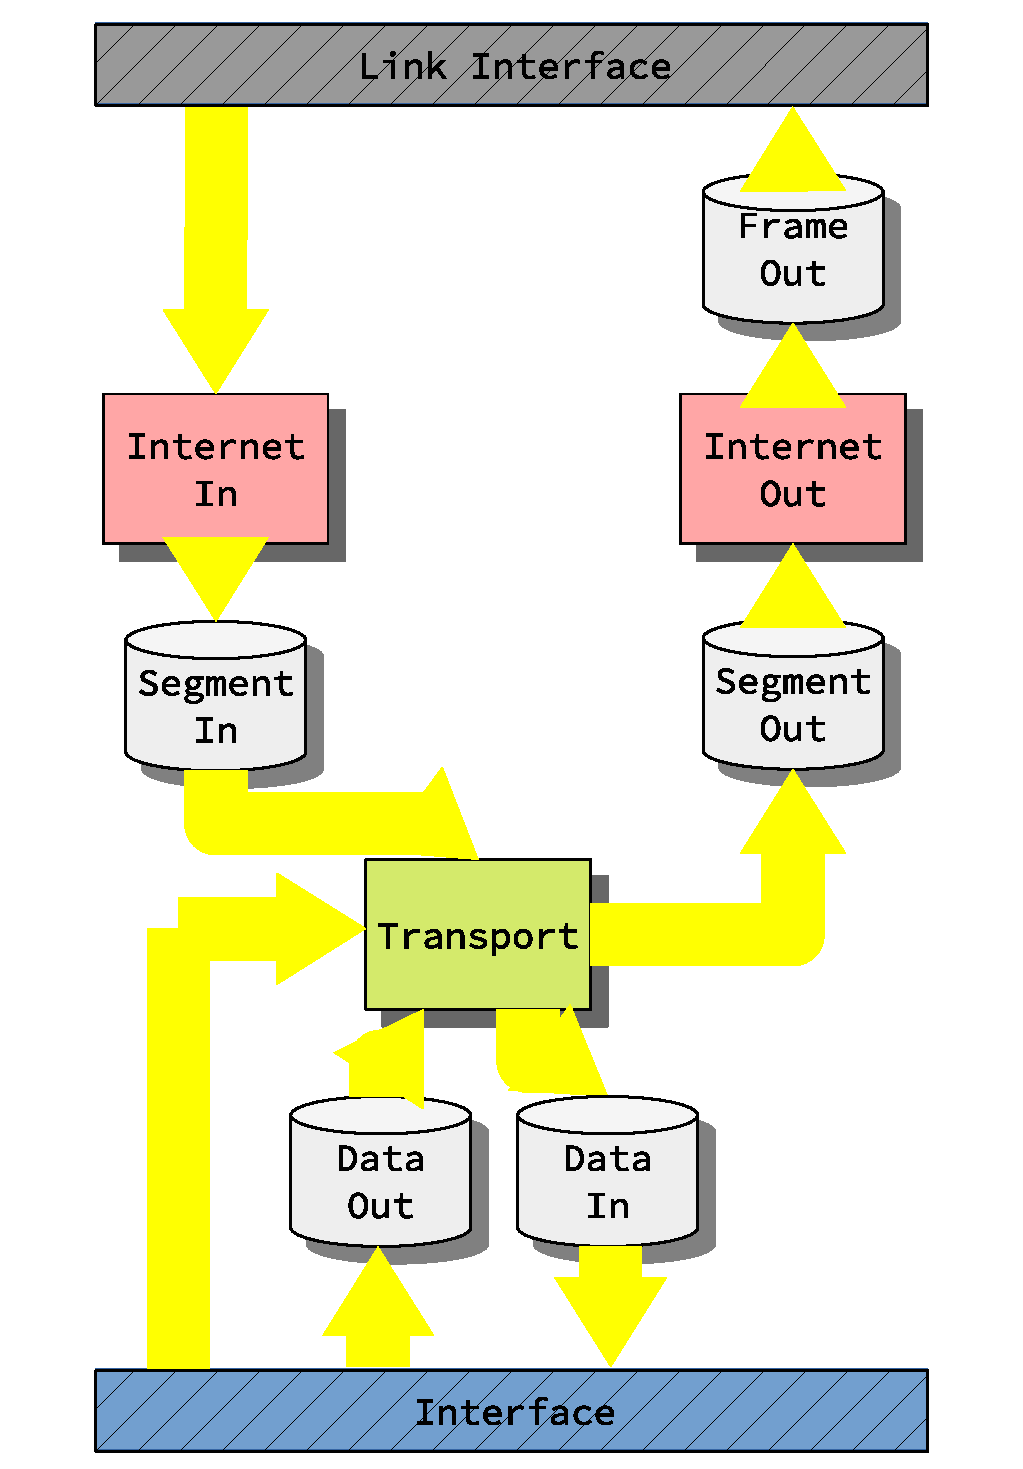
\includegraphics[width=\textwidth]{implementation/design_2_busses.eps}}
    \end{textblock*}
\frametitle{\ImplementationTitle}
\framesubtitle{Interface signal protocol}
\begin{figure}
        \centering
        \includegraphics[scale=0.35]{implementation/compute_producer.eps}
\end{figure}

\end{frame}




\begin{frame}[fragile]
    \begin{textblock*}{\displayThumbnail}(\paperwidth-\displayThumbnail-0.2cm,0cm) % {block width} (coords)
        \colorbox{white}{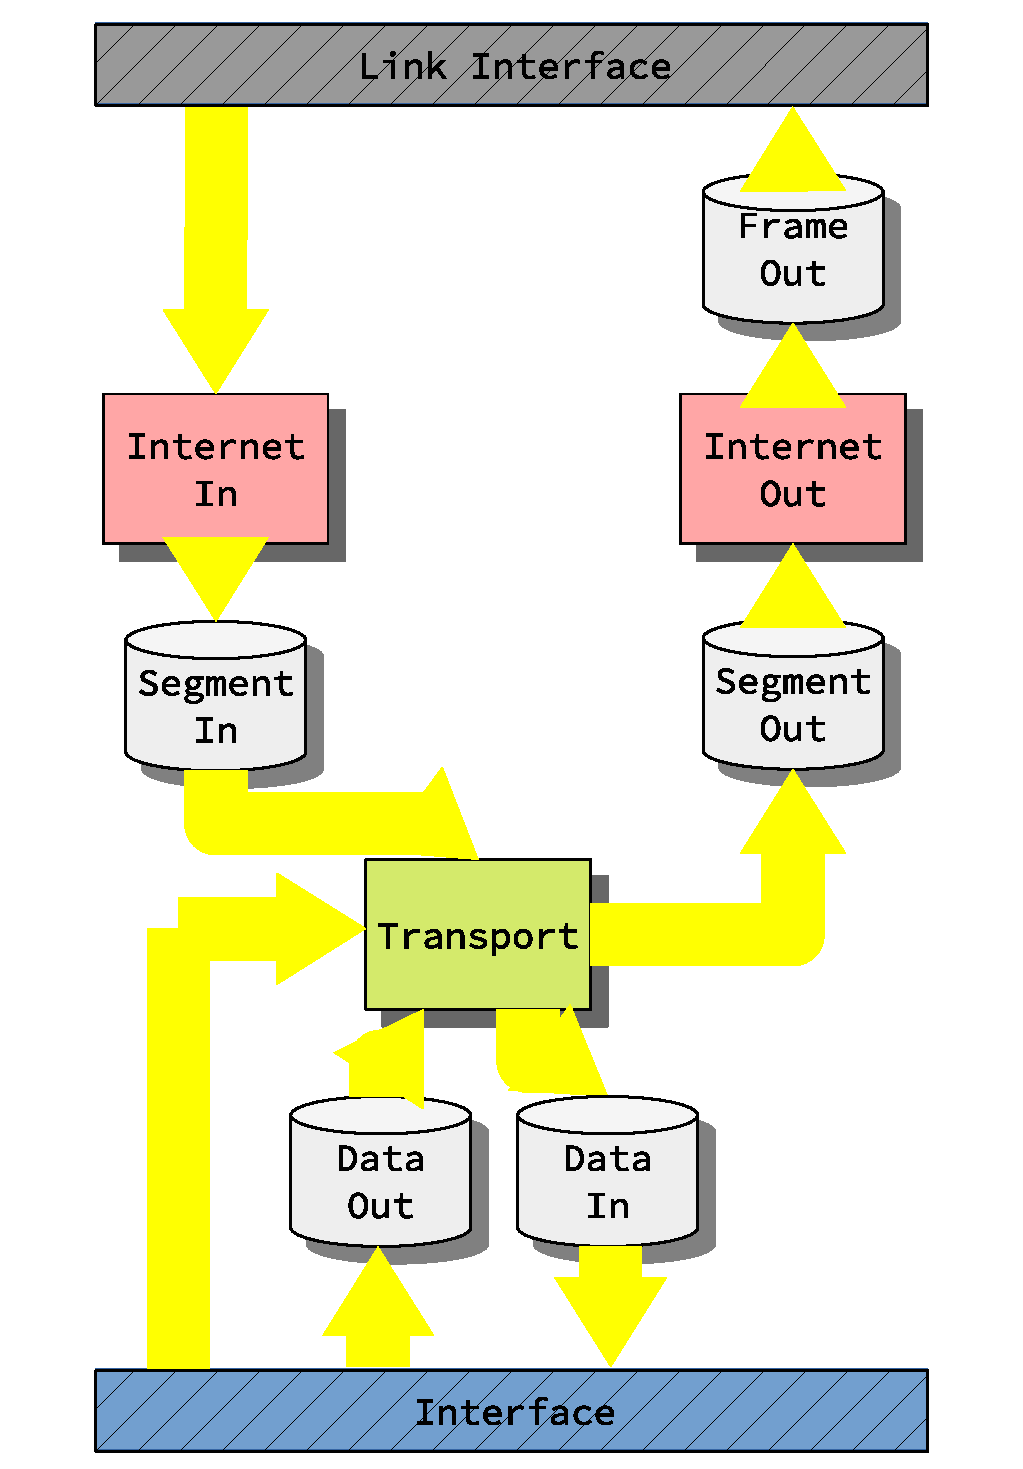
\includegraphics[width=\textwidth]{implementation/design_2_busses.eps}}
    \end{textblock*}
    \frametitle{\ImplementationTitle}
    \framesubtitle{Interface signal protocol}
    \textbf{Buffer-Producer:} Inspired by AXI4\\
    \begin{columns}
        \begin{column}{0.4\textwidth}
           \begin{itemize}
               \item Single clock offset when sending data.
               \item Indicate end of stream with \texttt{bytes\_left}.
           \end{itemize}
        \end{column}
        \begin{column}{0.5\textwidth}  %%<--- here
            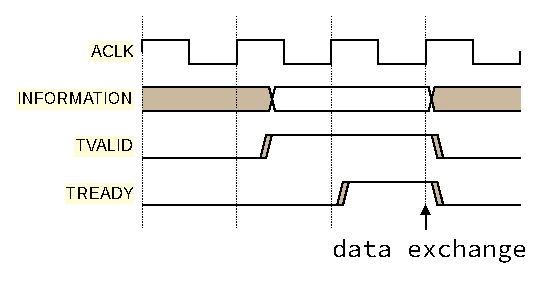
\includegraphics[scale=0.7]{implementation/axi4_handshake.eps}
        \end{column}
    \end{columns}
\end{frame}


\begin{frame}[fragile]
    \begin{textblock*}{\displayThumbnail}(\paperwidth-\displayThumbnail-0.2cm,0cm) % {block width} (coords)
        \colorbox{white}{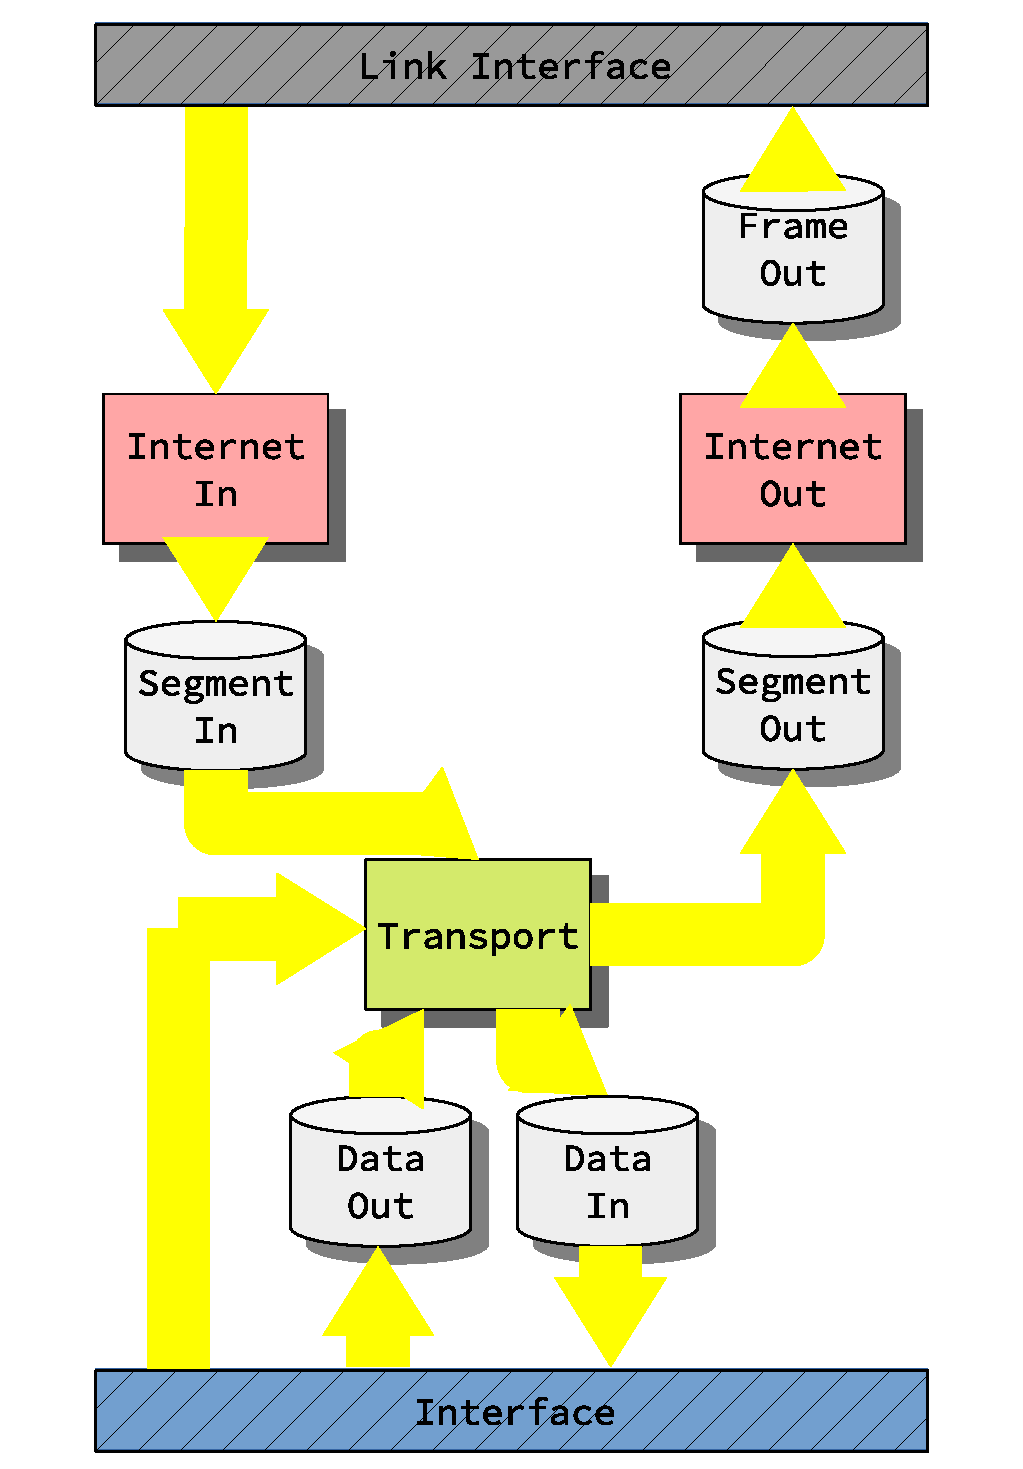
\includegraphics[width=\textwidth]{implementation/design_2_busses.eps}}
    \end{textblock*}
    \frametitle{\ImplementationTitle}
    \framesubtitle{Interface signal protocol}
        \begin{figure}
                \centering
                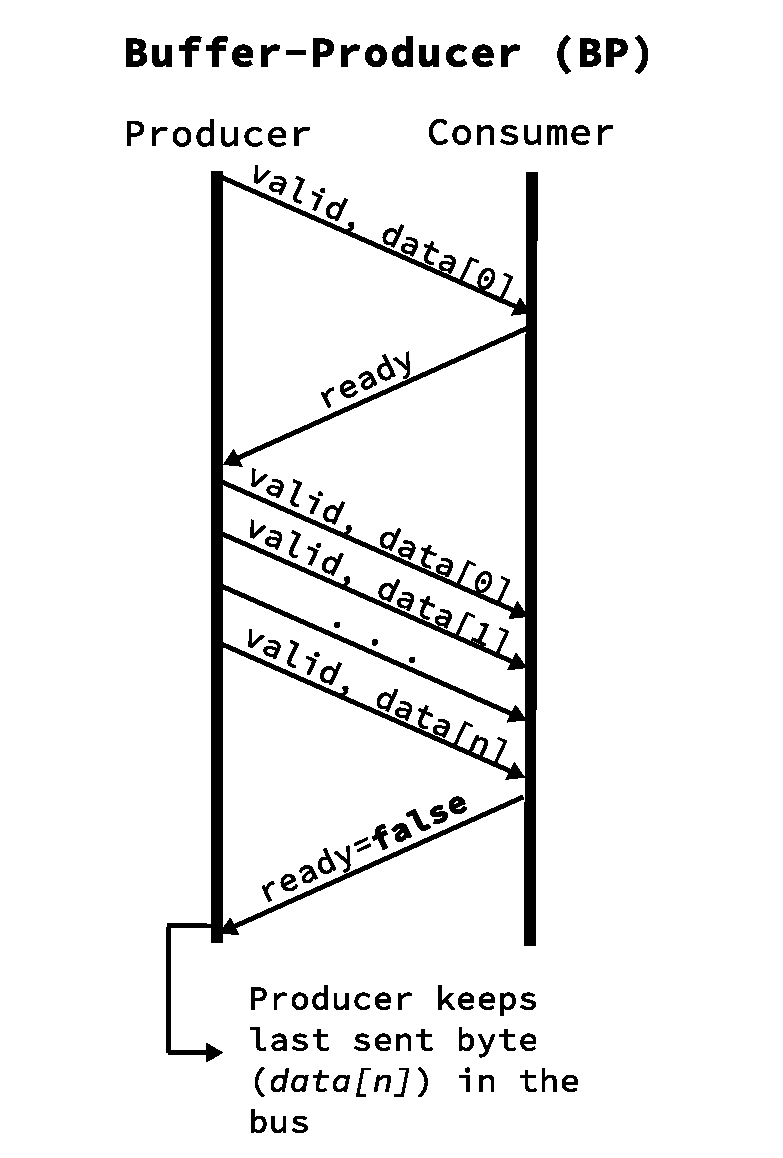
\includegraphics[scale=0.35]{implementation/buffer_producer.eps}
       \end{figure}
\end{frame}





% \begin{frame}[fragile]
%     \frametitle{\ImplementationTitle}
%     \framesubtitle{Interface protocol}
%     The interface structures\\
%     \begin{minipage}[t]{0.4\textwidth}
%         \begin{mintedcsharp}
%             enum InterfaceFunction : byte
%             {
%                 INVALID = 0,
%                 // BIND = 1,
%                 LISTEN = 2,
%                 CONNECT = 3,
%                 ACCEPT = 4,
%                 CLOSE = 7,
%                 // ...
%                 OPEN = 255,
%             }
%
%             struct InterfaceData
%             {
%                 public int socket;
%                 public uint ip;
%                 public byte protocol;
%                 public ushort port;
%             }
%         \end{mintedcsharp}
%     \end{minipage}%
%     \hfill%
%     \begin{minipage}[t]{0.4\textwidth}
%         \begin{mintedcsharp}
%             interface InterfaceBus : IBus
%             {
%                 bool valid;
%                 byte interface_function;
%                 InterfaceData request;
%             }
%
%             interface InterfaceControlBus : IBus
%             {
%                 bool valid;
%
%                 byte exit_status;
%                 byte interface_function;
%                 InterfaceData request;
%                 InterfaceData response;
%             }
%         \end{mintedcsharp}
%     \end{minipage}
% \end{frame}
%
%
% \begin{frame}%[fragile]
%     \frametitle{\ImplementationTitle}
%     \framesubtitle{Interface protocol}
%     Limitations
%     \begin{itemize}
%         \item One request at a time.
%         \item Arbitrary delay between request and response.
%     \end{itemize}
% \end{frame}
